\documentclass[11pt]{article}
\usepackage{fullpage}
\usepackage[T1]{fontenc}
\usepackage{lmodern}
\usepackage{amsmath,amssymb,amsthm,mathtools}
\usepackage{booktabs,array,microtype,needspace}
\usepackage{authblk}
\usepackage{tikz}
\usetikzlibrary{positioning,shapes.geometric,calc}
\usepackage{enumitem}
\usepackage[mathlines]{lineno}
\newif\ifreviewversion
\reviewversionfalse % Set true for line numbers; the page geometry is unchanged.
\ifreviewversion\linenumbers\fi
\usepackage[numbers,sort&compress]{natbib}
\usepackage[hidelinks]{hyperref}
\usepackage{bookmark}

% \hypersetup{pdftitle={An Exponential Succinctness Gap between Three-Variable Logic and the Calculus of Relations}}

\urlstyle{same}
\newcommand{\doi}[1]{\href{https://doi.org/#1}{\nolinkurl{doi:#1}}}
\allowdisplaybreaks[2]
\setlength{\parindent}{1.2em}
\setlength{\parskip}{0.15em}
\newtheorem{theorem}{Theorem}[section]
\newtheorem{lemma}[theorem]{Lemma}
\newtheorem{proposition}[theorem]{Proposition}
\newtheorem{corollary}[theorem]{Corollary}
\theoremstyle{definition}
\newtheorem{definition}[theorem]{Definition}
\theoremstyle{remark}
\newtheorem{remark}[theorem]{Remark}

\newcommand{\set}[1]{\{ #1 \}}
\newcommand{\cost}[1]{\#_{;}(#1)}
\newcommand{\gcost}[1]{g_{;}(#1)}
\newcommand{\CoR}{\ensuremath{\mathrm{CoR}}}
\newcommand{\FOtwo}{\ensuremath{\mathrm{FO}^{2}}}
\newcommand{\FOthree}{\ensuremath{\mathrm{FO}^{3}}}
\newcommand{\FOfour}{\ensuremath{\mathrm{FO}^{4}}}
\newcommand{\zero}{\mathbf{0}}             % the empty relation
\newcommand{\one}{\mathbf{1}}              % the full relation
\newcommand{\id}{\mathbf{1}'}              % the identity relation
\newcommand{\conv}{\smile}
\newcommand{\bool}{\mathbb B}
\newcommand{\wid}[1]{\mathsf{sn}(#1)}      % support number of a kernel or of a computation
\newcommand{\Arr}{\mathcal A_S}
% --- notation of the finite structure (Sections 3--6) ---
% Reserved letters.  Vertices: h (hub), u,v (general), z (witness),
% x (anchor).  Colors: lambda, mu, nu in \Col; for the two hard formulas a
% color is a subset A,B of [k].  Cells: C_lambda, C_J, C_\Col -- always
% subscripted, so that \Comp = \mathcal C, a computation, is never
% ambiguous.  The coloring is \colr = chi.  The kernel of an aggregation is
% the infix \odot, so that psi is free and Psi_k unambiguous; its width is
% \wid.
\newcommand{\Col}{\Lambda}                 % set of colors
\newcommand{\colr}{\chi}                   % the coloring of the core edges
\newcommand{\cell}[1]{C_{#1}}              % cell of color #1; also C_J, C_\Col
\newcommand{\Comp}{\mathcal C}             % a computation / relational circuit
\newcommand{\ctype}[1]{\tau_{#1}}          % type: edges of color #1
\newcommand{\tpa}[2]{\tau_{#1,#2}}         % type: the anchor pair (#1,#2)
\newcommand{\tpl}[1]{\tau_{#1,\ast}}       % type: anchor #1 to a core vertex
\newcommand{\tpr}[1]{\tau_{\ast,#1}}       % type: a core vertex to anchor #1
\newcommand{\tpeq}{\tau_{=}}               % type: loops of core vertices
\newcommand{\tp}{\operatorname{tp}}        % type of a pair
\newcommand{\agg}[1]{\mathbin{;_{#1}}}     % aggregation with kernel #1
\newcommand{\res}{\mathord{\restriction}}  % restriction
\newcommand{\M}{\mathfrak M}               % reference structure
\newcommand{\A}{\mathfrak A}               % an arbitrary structure
\newcommand{\Det}{\Lambda_0}               % detectable colors
\newcommand{\breadth}{\beta}               % join breadth of a semiring
\newcommand{\cd}[1]{e_{#1}}                % the code of a bit
\newcommand{\cdb}{e_{\bot}}                % the invalid code
\newcommand{\prof}{\operatorname{prof}}    % the profile of a type (Remark 4.1)
\newcommand{\num}{\operatorname{num}}      % the number of a subset
\newcommand{\ind}{\operatorname{ind}}      % discrete logarithm mod N
% Part headings: one line each, no page break, no interaction with section numbering.
\newcommand{\partheading}[2]{%
  \par\bigskip\noindent{\large\bfseries Part #1: #2}\par\nobreak\medskip}
\title{An Exponential Succinctness Gap between\protect\\Three-Variable Logic and the Calculus of Relations}

\author{Yuya Uezato}
\affil{CyberAgent, Inc., uezato\_yuya@cyberagent.co.jp}

\if0
\author[1]{Yuya Uezato}
\author[2]{Yoshiki Nakamura}
\affil[1]{CyberAgent, Inc., uezato\_yuya@cyberagent.co.jp}
\affil[2]{Chiba University, nakamura.yoshiki.ny@gmail.com}
\fi

\date{}
\begin{document}
\maketitle
\begin{abstract}
Three-variable first-order logic ($\mathrm{FO}^{3}$) and the calculus of relations ($\mathrm{CoR}$) define the same binary queries, an equivalence going back to Tarski in the 1940s.
%
While the classical translation $\mathrm{FO}^{3}\Rightarrow\mathrm{CoR}$ is exponential, we prove that this blow-up is unavoidable, resolving a long-standing open question.
%
We construct positive formulas $\varphi$ with a single quantifier whose equivalent terms require size $2^{\Omega(|\varphi|)}$, even over finite structures and circuit representations with subterm sharing.
%
Our proof uses a preservation argument over a single finite structure.
This approach applies beyond our primary question, establishing the lower bound even for size-specific circuits and bounded-error randomized circuits, and yielding an analogous exponential gap for the matrix query language MATLANG.
\end{abstract}
\section{Introduction}
Three-variable first-order logic ($\FOthree$) over binary relations and the
calculus of relations
(\CoR) define the same binary queries, an equivalence going back to
Tarski's 1940s work~\citep{tarski-givant1987}. \CoR\ is the algebra of
binary relations under union $P\cup Q$, intersection $P\cap Q$, complement
$\overline P$, converse $P^\smile=\set{(y,x):(x,y)\in P}$, and the
composition, or relative product,
$P;Q=\set{(x,y):\exists z.\,(x,z)\in P,\ (z,y)\in Q}$. \CoR\ has no
individual variables, so quantifier elimination has to go through the
composition:
\begin{equation}\label{eq:basic-identity}
 \exists z\,\bigl(P(x,z)\land Q(z,y)\bigr)\iff(P;Q)(x,y).
\end{equation}
Using \eqref{eq:basic-identity} together with bottom-up disjunctive normal
form (DNF)
conversion~\citep{hilbert-ackermann1928,kleene1952,schoening1989},
$\FOthree$ formulas can be translated into \CoR\ with a single-exponential
blow-up. Both were in place before Tarski took up the question
(see Section~\ref{sec:relwork}). For an example, fix $k\ge2$ and consider the
$\FOthree$ formula
\begin{equation}\label{eq:omega}
\Psi_k(x,y) := \exists z\,\bigwedge_{i=1}^k
       \bigl(R_i(x,z)\lor R_i(z,y)\bigr),
\end{equation}
which asks for a single witness $z$ satisfying $R_i(x,z)\lor R_i(z,y)$ for
every $i\in\{1,\dots,k\}$. To apply \eqref{eq:basic-identity}, the body
under the quantifier must be factored into the form
$\alpha(x,z)\land\beta(z,y)$. Thus, by DNF conversion, the body of
\eqref{eq:omega} expands into $2^k$ disjuncts, one for each subset
$I\subseteq[k]$, the disjunct for $I$ asserting that $R_i(x,z)$ holds for
$i\in I$ and $R_i(z,y)$ for $i\notin I$. Applying
\eqref{eq:basic-identity} to each disjunct gives an equivalent \CoR\ term of
size $2^{O(k)}$,
\begin{equation}\label{eq:omega-upper}
 \CoR_{\Psi_k} := \bigcup_{I\subseteq[k]}
 \biggl(\Bigl(\bigcap_{i\in I}R_i\Bigr);\Bigl(\bigcap_{i\notin I}R_i\Bigr)\biggr),
\end{equation}
where an empty intersection denotes the full relation $\one$, which holds at
every pair. For $k=3$ the eight choices of $I$ give eight disjuncts and
eight compositions:
\[
\renewcommand{\arraystretch}{1.15}
\begin{array}{c@{\qquad}l@{\qquad}l}
 I&\text{disjunct of the DNF}&\text{term}\\\hline
 \{1,2,3\}&R_1(x,z)\land R_2(x,z)\land R_3(x,z)&(R_1\cap R_2\cap R_3);\one\\
 \{1,2\}&R_1(x,z)\land R_2(x,z)\land R_3(z,y)&(R_1\cap R_2);R_3\\
 \{1,3\}&R_1(x,z)\land R_3(x,z)\land R_2(z,y)&(R_1\cap R_3);R_2\\
 \ \ \vdots&\qquad\qquad\vdots&\qquad\ \ \vdots\\
 \varnothing&R_1(z,y)\land R_2(z,y)\land R_3(z,y)&\one;(R_1\cap R_2\cap R_3)
\end{array}
\]
That the translation is exponential in general is classical.
\begin{proposition}[well known; see Section~\ref{sec:relwork}]\label{prop:upper-translation}
Every \FOthree\ formula $\varphi$ over binary relations with at most two
free variables is
equivalent, on all structures, to a \CoR\ term of size $2^{O(|\varphi|)}$,
where $|\cdot|$ counts the nodes of a syntax tree.
\end{proposition}

Whether this single-exponential upper bound is optimal has remained a
long-standing open question, and no matching lower bound for full \CoR\ has
been known since the correspondence itself was established.

In this paper we prove that the blow-up is unavoidable: the
$2^{\Omega(|\varphi|)}$ lower bound holds already over finite structures,
already for positive \FOthree\ formulas with a single quantifier, and even
when the \CoR\ side is a circuit rather than a term.

\subsection{Main results}\label{sec:main-results}
Write $|\varphi|$ and $|t|$ for the number of nodes in the syntax tree of a
formula $\varphi$ or a term $t$, and $\cost{t}$ for the number of
\emph{composition} nodes of $t$; in the second measure the Boolean
operations and converse are free. A \emph{relational circuit} $\Comp$ is a
term whose subterms may be shared, that is, a directed acyclic graph, and
$\gcost{\Comp}$ counts its distinct composition gates. Write
$t\equiv_{\rm fin}\varphi$ if $t$ and $\varphi$ define the same relation on
every finite structure, and likewise for circuits. The first hard query is
$\Psi_k$ itself, and the $2^k$ compositions of \eqref{eq:omega-upper} are
close to necessary.

\begin{theorem}[Disjunctive clauses]\label{main:omega}
Let $k\ge2$. Every \CoR\ term $t\equiv_{\rm fin}\Psi_k$ satisfies
\[
 \cost{t}\ \ge\ \Bigl\lceil\tfrac12\binom{k}{\lfloor k/2\rfloor}\Bigr\rceil
 \qquad\text{and}\qquad
 |t|\ \ge\ \binom{k}{\lfloor k/2\rfloor}+1,
\]
and the bound on $\cost{t}$ holds more generally for circuits: every
relational
circuit $\Comp\equiv_{\rm fin}\Psi_k$ has
$\gcost{\Comp}\ge\bigl\lceil\frac12\binom{k}{\lfloor k/2\rfloor}\bigr\rceil$.
\end{theorem}

Since $\binom{k}{\lfloor k/2\rfloor}=\Theta(2^k/\sqrt k)$, this falls short
of the $2^k$ compositions of \eqref{eq:omega-upper} by a factor of
$\Theta(\sqrt k)$. The second hard query closes the gap. It asks
the two pairs $(x,z)$ and $(z,y)$ to satisfy the
same one of two symbols in each clause, rather than to share out the $k$
clauses between them. For $k\ge1$
let
\begin{equation}\label{eq:phi}
\Phi_k(x,y) := \exists z\,\bigwedge_{i=1}^k
       \Bigl(\bigl(P_i(x,z)\land P_i(z,y)\bigr)\lor
             \bigl(Q_i(x,z)\land Q_i(z,y)\bigr)\Bigr),
\end{equation}
over the $2k$ independent symbols $P_1,Q_1,\ldots,P_k,Q_k$. Clause $i$ holds
at a witness $z$ when both edges $(x,z)$ and $(z,y)$ lie in $P_i$, or both
lie in $Q_i$.

\begin{theorem}[Profile agreement]\label{main:phi}
Let $k\ge1$. Every \CoR\ term $t\equiv_{\rm fin}\Phi_k$ satisfies
$\cost{t}\ge2^{k-1}$ and $|t|\ge2^k+1$, and the bound on $\cost{t}$ holds
more
generally for circuits: every relational circuit
$\Comp\equiv_{\rm fin}\Phi_k$ has $\gcost{\Comp}\ge2^{k-1}$. The explicit
term $\CoR_{\Phi_k}$ of \eqref{eq:phi-upper} uses $2^k$ compositions, so the
composition count
is determined within a factor of two.
\end{theorem}

Both formulas are positive, use a single quantifier, and have size
$\Theta(k)$ over a vocabulary that grows with $k$
(Remark~\ref{rem:vocabulary}), so the two theorems answer the question
above.

\begin{corollary}[Succinctness gap]\label{cor:gap}
The translation of Proposition~\ref{prop:upper-translation} is optimal up to
the constant in the exponent: there are positive \FOthree\ formulas
$\varphi$ with one quantifier, of arbitrarily large size, such that every
relational circuit equivalent to $\varphi$ over finite structures has size
$2^{\Omega(|\varphi|)}$.
\end{corollary}
\begin{proof}
Take $\varphi=\Psi_k$, of size $\Theta(k)$. By Theorem~\ref{main:omega} a
circuit for it has at least $\frac12\binom{k}{\lfloor k/2\rfloor}$
composition gates, and $\binom{k}{\lfloor k/2\rfloor}\ge2^k/(k+1)$, so its
size is at least $2^{k-O(\log k)}=2^{\Omega(|\varphi|)}$, while
\eqref{eq:omega-upper} is an equivalent term of size
$O(k2^k)=2^{O(|\varphi|)}$. Taking $\varphi=\Phi_k$
gives $2^k$ in place of $2^k/(k+1)$.
\end{proof}

Section~\ref{sec:overview} outlines the proof of
Theorem~\ref{main:omega}, which works also for Theorem~\ref{main:phi}.

What Corollary~\ref{cor:gap} leaves open is the same question over a
vocabulary \emph{fixed} in advance. The formulas above use $k$ and $2k$
relation symbols respectively,
and $|\varphi|=\Theta(k)$ because the size charges an occurrence of a symbol
one node. Over a single binary relation symbol we obtain, for positive formulas, a gap of
$2^{\Omega(n/\log n)}$ (Theorem~\ref{thm:af-fixed}); whether $2^{\Omega(n)}$
holds over a fixed vocabulary we do not know
(Remark~\ref{rem:vocabulary}).

\subsection{Additional results}\label{sec:additional-results}

\paragraph{Size-specific and randomized targets.}
A \CoR\ term is a single expression, evaluated on structures of every size,
so Theorems~\ref{main:omega} and~\ref{main:phi} are uniform lower bounds.
The same bounds hold non-uniformly, with the term or circuit chosen for each
domain size $n$, and a bounded probability of error costs only a constant
factor.

\begin{theorem}[informal; see Theorem~\ref{thm:fixed-size} and
Corollary~\ref{cor:randomized}]\label{main:robust}
Let $\varphi$ be $\Psi_k$ or $\Phi_k$. For every $n$ above a threshold
$n_0=2^{O(k)}$, the lower bounds of Theorems~\ref{main:omega}
and~\ref{main:phi} hold for every term or circuit that agrees with $\varphi$
on all structures with exactly $n$ elements, even when that term is chosen
depending on $n$. A randomized circuit that is correct with probability at
least $1-\varepsilon$ on every input, for some $\varepsilon<1/2$, still
needs a $(1-2\varepsilon)$ fraction of that same number of compositions, in
expectation.
\end{theorem}

\paragraph{Matrix query languages.}
The composition $P;Q$ can be replaced by $\bigvee_zP(x,z)\odot Q(z,y)$, with
$\odot$ an arbitrary binary operation on the scalars and $\bigvee$ an
arbitrary idempotent join (Section~\ref{sec:responses}), and the lower
bounds continue to hold; the min-plus matrix product
$\min_z\bigl(P(x,z)+Q(z,y)\bigr)$ is one instance. \citet{brijder2022}
showed that MATLANG defines the same binary queries as a positive
relational algebra on semiring-annotated relations whose intermediate
results have at most three attributes; their translation into MATLANG is
exponential, and they asked whether that blow-up is unavoidable.

\begin{theorem}[informal; see Theorem~\ref{main:matrix}, and
Corollary~\ref{cor:positive} for non-idempotent semirings]\label{main:matrix-informal}
Fix the min-plus semiring, or max-plus, or max-min. For every $k$ there is a
positive relational algebra expression $E_k$ of size $O(k)$, with binary
output, whose intermediate results have at most three attributes. Every
MATLANG computation equivalent to $E_k$ on $n\times n$ inputs uses at least
$2^k/3$ matrix products contracting the dimension $n$, even with arbitrary
uniform entrywise functions and shared intermediates; $2^k$ products
suffice.
\end{theorem}

\subsection{Related work}\label{sec:relwork}

\paragraph{The expressiveness question.}
For historical background, we refer to the surveys by \citet{pratt1992},
\citet{maddux1991}, and \citet{burris-legris}, the monograph of
\citet{brady2000}, and the historical notes of \citet{tarski-givant1987}.
\CoR\ is older than first-order logic. De Morgan introduced composition
and converse in his papers on the syllogism of 1850 and
1860~\citep{demorgan1856,demorgan1864}, Peirce developed the algebra
through the 1870s and 1880s~\citep{peirce1870,peirce1880}, and Schr\"oder
devoted an entire volume to it in 1895~\citep{schroeder1895}. In contrast,
first-order logic was formalized only in Hilbert's lectures of 1917--18 and
in Hilbert and Ackermann's 1928
book~\citep{hilbert-lectures,hilbert-ackermann1928,moore1988}. In the
terminology of the time, to \emph{condense} a quantified statement about
relations meant eliminating its quantifiers to express it within the
calculus~\citep[p.~233]{loewenheim1915}---the translation of
Proposition~\ref{prop:upper-translation} under its older name. Schr\"oder
claimed in 1895 that every such statement could be
condensed~\citep[p.~551]{schroeder1895}. Korselt found a counterexample,
published by L\"owenheim in 1915~\citep{loewenheim1915}, which lies
exactly on the variable boundary studied here: ``the domain has at most two
elements'' requires three variables (\FOthree) and can be condensed,
whereas ``the domain has at most three elements'' requires four (\FOfour) and
cannot. Statements in \FOfour\ were thus known to lie outside \CoR\
before first-order logic existed as a formal system, while the status of
\FOthree\ remained open.
Tarski's 1941 paper presented further
\FOfour\ statements outside \CoR,
observed that the calculus remained at essentially the same stage of development as forty-five years earlier,
and posed the problem of characterizing the
condensable sentences~\citep[pp.~74, 89]{tarski1941}.
According to Tarski and
Givant, Tarski obtained the \FOthree\ characterization in the early 1940s
and presented it at a 1945 Berkeley seminar. It was first published with full
proofs in their 1987 monograph~\citep[pp.~xvii, 88--89]{tarski-givant1987},
and Maddux provided a modern treatment in his monograph~\citep{maddux2006}.
This settled the expressiveness question and forms the basis for
Proposition~\ref{prop:upper-translation} and Corollary~\ref{cor:gap},
but the computational cost of this translation was not examined.

\paragraph{The succinctness question.}
Expressive equivalence, however, implies nothing about formula size. Tarski
and Givant defined their translation recursively, providing no bound on its
growth~\citep[\S3.9]{tarski-givant1987}. The folklore translation behind
Proposition~\ref{prop:upper-translation} applies bottom-up DNF conversion to
the quantifier-free Boolean shell of a formula---the propositional normal-form
theorem of \citet{hilbert-ackermann1928}, read as a conversion procedure by
\citet{kleene1952} and \citet{schoening1989}---and then applies
\eqref{eq:basic-identity} to each disjunct. This bottom-up conversion is
the sole source of the exponential blow-up. In contrast, the reverse
translation is linear: structural induction turns a \CoR\ term of size $m$
into an \FOthree\ formula of size $O(m)$, so the blow-up occurs in one
direction only. Whether this exponential blow-up is unavoidable has remained
open since the equivalence was established. The query $\Psi_k$ is due to
\citet{nakamura2022}, who showed that it has no subexponential translation
into \emph{positive} \CoR\ (the fragment without complement), leaving the
case of full \CoR\ open. Theorems~\ref{main:omega} and~\ref{main:phi} settle
this question.

\paragraph{Succinctness of logics and lower-bound methods.}
Succinctness is a standard measure for comparing logics of the same
expressive power~\citep{grohe-schweikardt2005}, and gaps of every size are
known between fragments of first-order, temporal, and modal
logics~\citep{etessami-vardi-wilke2002,adler-immerman2003,dawar2007,french2013}.
The closest result to ours concerns finite-variable fragments over a
single binary relation: on finite linear orders, \FOfour\ is
exponentially more succinct than \FOthree, while two- and three-variable
logics are polynomially equivalent~\citep{grohe-schweikardt2005}. Such lower
bounds are proved using the formula-size games of Adler and
Immerman~\citep{adler-immerman2003,hella-vilander2019} or, equivalently, by
tracking a potential function along syntax trees~\citep{grohe-schweikardt2005}.
This framework is indifferent to negation (which merely swaps structure pairs)
and charges a bounded potential increase for each quantifier (corresponding
to composition in \CoR). The core difficulty lies in finding suitable
structures and a potential, neither of which transfers from linear orders to
our setting, for two concrete reasons.

First, on linear orders there is no gap to find: by the lower-bound theorem of
Grohe and Schweikardt~\citep{grohe-schweikardt2005}, an \FOthree\ formula of
size $s$ can only tell in which order its points come and whether two of
them lie at distance exactly $d$ for some $d\le4s^2$, and each such test is
a \CoR\ term of size $O(d)$, namely a $d$-fold composition of
$\mathit{succ}=(<)\cap\overline{(<\,;<)}$. As a formula of size $s$ is a
Boolean combination of the $s^{O(1)}$ available tests, it has an equivalent
\CoR\ term of size $s^{O(1)}$; so \FOthree\ and \CoR\ terms are
polynomially equivalent there.

Second, the mechanism of their gap is fundamentally different. A fourth variable
permits the divide-and-conquer recursion familiar from Savitch's theorem~\citep{savitch1970},
\[
 \varphi_m(x,y) = \exists z\,\forall u\,\bigl((u=x\lor u=y)\to
 \varphi_{m-1}(z,u)\bigr),
\]
which expresses ``$x$ and $y$ are at distance $2^m$'' in size $O(m)$ by
using one copy of $\varphi_{m-1}$ for both halves of the
path~\citep{grohe-schweikardt2005}; with three variables the recursion must
write $\varphi_{m-1}$ twice at every level, and their lower bound shows
that no other \FOthree\ formula does better than $2^{\Omega(m)}$.
Reuse is exactly what a circuit provides: a relational circuit expresses
distance $2^m$ with $m$ compositions, by squaring $S_{i+1}=S_i;S_i$ from
$S_0=\mathit{succ}$, whereas a term needs size $2^{\Omega(m)}$ by their
bound and the linear translation of terms into \FOthree. Our bounds hold for
circuits---where on linear orders the gap actually runs in the opposite
direction---showing that the gap between \FOthree\ and \CoR\ is not simply
one of reuse.

This gap stems from how the two formalisms handle witnesses: in $\Psi_k$, the
quantifier binds $R_i(x,z)\lor R_i(z,y)$ for all $i$ simultaneously,
constraining both edges at once. In contrast, a composition $P;Q$ splits the
edges into $P$ and $Q$. The classical translation \eqref{eq:omega-upper} must
therefore spend one composition on each way of partitioning the $k$ clauses
between the two edges, an overhead that Theorem~\ref{main:omega} proves to be
unavoidable. \citet{nakamura2022} proved the exponential bound for positive
\CoR\ using a formula-size game; however, the argument relies fundamentally on
positivity and does not extend to complement, which exchanges the two sides
and thus requires a symmetric potential. Our preservation theorem supplies
one: for a single finite structure and the family of substructures obtained by
deleting one part each, the potential of a subterm is a set of parts outside
of which every deletion is invisible to it. Boolean operations and converse
contribute nothing to this set, while a composition contributes at most two
parts; because these parts combine by union rather than by addition, a shared
gate is charged only once, directly yielding the bound for circuits. Finally,
$\Psi_k$ and $\Phi_k$, suitably interpreted, detect every deletion.

\paragraph{Composition as matrix multiplication.}
Since composition corresponds to a Boolean matrix product, a \CoR\ term with $m$
compositions evaluates a query using $m$ fast matrix multiplications in time
$O(m\,n^{\omega})$, rather than the $O(n^3)$ time of naive enumeration,
where $\omega$ is the matrix multiplication exponent. Bounded-variable queries
can be evaluated in time polynomial in both the query and the
structure~\citep{vardi1995}. \citet{Williams2014} exploited this speedup for
three-quantifier graph properties, leading to a fine-grained complexity
theory of first-order queries parameterized by variable count and quantifier
structure~\citep{GaoImpagliazzoKolokolovaWilliams2017,BringmannFischerKunnemann2019,GaoImpagliazzo2019}.
The composition counts in Theorems~\ref{main:omega} and~\ref{main:phi}
therefore lower-bound the number of matrix products required by any
relational evaluation of the query, a bound stated directly in
Theorem~\ref{main:matrix}. These results are not lower bounds for general
Boolean circuits with access to individual input entries. In our cost measure,
all Boolean operations (including complement) are free. In contrast,
classical monotone lower bounds for a single Boolean matrix
product~\citep{kerr1970,pratt1975,paterson1975,mehlhorn-galil1976} and
exact bounds for straight-line programs over semirings~\citep{jerrum-snir1982}
count individual gates; see \citet{jukna2012} for a survey.

\paragraph{Relational and matrix query languages.}
Algebraic representations of logical queries have been central to query
processing since Codd~\citep{Codd1970,Codd1972}. Binary relation algebra and its
fragments form the algebraic core of graph and navigational query
languages~\citep{FletcherEtAl2015,HellingsEtAl2021,HellingsEtAl2022}. In these
settings, logic-to-algebra translations can incur exponential
blowups~\citep{BaranyTenCateOtto2012}. The succinctness of relational
representations is therefore a central concern~\citep{FletcherEtAl2015},
because the size of the translated expression directly dictates the cost of
query optimization and evaluation. MATLANG is a matrix query language built
from matrix multiplication, transpose, ones-vectors, diagonalization, and
pointwise functions~\citep{brijder2019tods}; see \citet{geerts2021} for a
survey. For relations annotated with values in a semiring, in the sense of
provenance semirings~\citep{green2007},
\citet{brijder2022} proved that binary-output ARA(3)---the three-attribute
annotated relational algebra---is expressively equivalent to MATLANG,
mirroring the equivalence between \FOthree\ and \CoR. An earlier manuscript
asked whether this exponential arity elimination (and by analogy, the
classical \FOthree\ translation) is unavoidable~\citep[p.~9]{brijder2019}.
Theorem~\ref{main:matrix} resolves this question affirmatively for
commutative idempotent semirings of finite join breadth, while
Section~\ref{semi:positive-section} extends the bound to additional semirings
under a restricted operation set.


\subsection{Technical overview}\label{sec:overview}
We outline the proof of Theorem~\ref{main:omega}. Theorem~\ref{main:phi}
uses the same construction and the same preservation theorem, and differs
only in the interpretation of the relation symbols.

\subsubsection{Outline}\label{ov:outline}
The term \eqref{eq:omega-upper} contains one composition for each way of
distributing the $k$ clauses between the two edges of the witness. A more
economical term might use complementation, factor out common subterms, or
share them, and a normal-form argument would have to account for all of
these possibilities. We therefore do not analyze the syntax of a candidate
term at all. Instead, we fix a single finite structure, delete parts of it,
and ask which of the resulting substructures a given term can still
distinguish from the original.

We say that a term or a query \emph{distinguishes} two structures over the
same vocabulary, one of them a substructure of the other, if the relations
that it defines on them differ at some pair of vertices of the smaller
structure; equivalently, the term or query \emph{detects} the deletion that
produced the smaller structure. The proof has three steps.
\begin{enumerate}[nosep,label=(\roman*)]
\item We build one finite structure $\M$ (Figure~\ref{fig:structure}).
 Apart from a hub and some anchors, its vertices are partitioned into
 \emph{cells} $\cell\lambda$, one for each color $\lambda$ in a finite set
 $\Col$ of at least two colors. The only substructures we use are those
 obtained by deleting entire cells: for nonempty $J\subseteq\Col$, let
 $\M\res J$ be $\M$ with every cell $\cell\lambda$ such that
 $\lambda\notin J$ removed. Thus no vertex is ever removed individually,
 and the hub and the anchors survive every deletion.
\item To a \CoR\ term $t$ with $m$ compositions we attach a set
 $K\subseteq\Col$ of at most $2m$ colors, and show that $t$ does not
 distinguish $\M$ from $\M\res J$ for any nonempty $J\supseteq K$
 (Theorem~\ref{thm:preservation}): deleting cells is invisible to $t$ as
 long as every cell whose color lies in $K$ is retained.
\item We interpret the relation symbols of $\Psi_k$ on $\M$ so that
 $\Psi_k$ does distinguish $\M$ from $\M\res(\Col\setminus\{\lambda\})$, for
 every single color $\lambda$ (Section~\ref{sec:logical}).
\end{enumerate}
Suppose $t\equiv_{\rm fin}\Psi_k$, and let $\lambda$ be any color. By~(iii)
the formula distinguishes $\M$ from $\M\res(\Col\setminus\{\lambda\})$, and
hence so does $t$. Since $|\Col|\ge2$, the set $\Col\setminus\{\lambda\}$ is
nonempty, so by~(ii) this is possible only if
$\Col\setminus\{\lambda\}\not\supseteq K$, that is, only if $\lambda\in K$.
Hence $K=\Col$ and $2m\ge|\Col|$. Taking for $\Col$ the $\lfloor
k/2\rfloor$-element subsets of $[k]$ gives the composition bound of
Theorem~\ref{main:omega}; the bound on $|t|$ follows from
\eqref{eq:tree-size}.

The remainder of this section treats the three steps in order.
Section~\ref{ov:structure} constructs $\M$ and specifies the pairs of
vertices at which a query is read off; Sections~\ref{ov:types}
to~\ref{ov:wholeterm} prove~(ii) by showing that what a term computes on
$\M$ is too coarse to detect an individual cell; and
Section~\ref{ov:formula} establishes~(iii).

\begin{figure}[t]
\centering
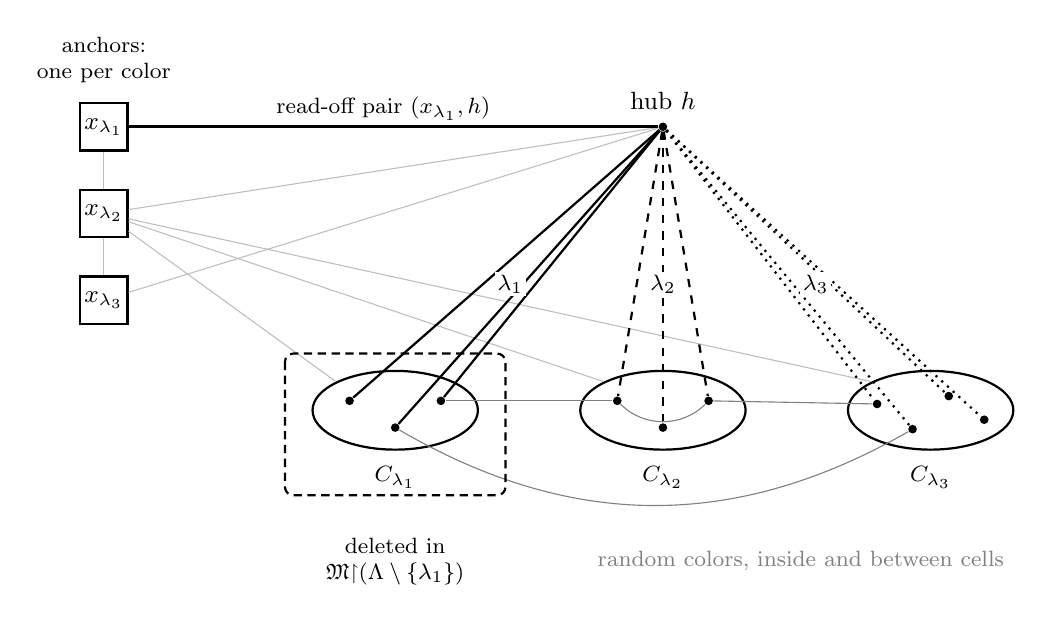
\begin{tikzpicture}[
  font=\small,
  cellnode/.style={draw,ellipse,minimum width=2.1cm,minimum height=1.0cm,thick},
  vtx/.style={circle,fill=black,inner sep=1.1pt},
  anch/.style={draw,rectangle,thick,minimum size=6mm,fill=white,inner sep=1pt}
]
 % ---------- hub ----------
 \node[vtx,label={[label distance=1pt]above:{hub $h$}}] (hub) at (0.4,3.6) {};
 % ---------- cells ----------
 \node[cellnode] (c1) at (-3.0,0) {};
 \node[cellnode] (c2) at ( 0.4,0) {};
 \node[cellnode] (c3) at ( 3.8,0) {};
 \node[below=2pt of c1,font=\footnotesize] {$\cell{\lambda_1}$};
 \node[below=2pt of c2,font=\footnotesize] {$\cell{\lambda_2}$};
 \node[below=2pt of c3,font=\footnotesize] {$\cell{\lambda_3}$};
 \foreach \c in {1,2}{
   \node[vtx] (c\c a) at ($(c\c)+(-0.58,0.12)$) {};
   \node[vtx] (c\c b) at ($(c\c)+(0.0,-0.22)$) {};
   \node[vtx] (c\c c) at ($(c\c)+(0.58,0.12)$) {};
 }
 % four dots in the third cell: the number drawn carries no meaning
 \node[vtx] (c3a) at ($(c3)+(-0.68,0.08)$) {};
 \node[vtx] (c3b) at ($(c3)+(-0.23,-0.24)$) {};
 \node[vtx] (c3c) at ($(c3)+(0.23,0.18)$) {};
 \node[vtx] (c3d) at ($(c3)+(0.68,-0.12)$) {};
 % ---------- anchors: one per color ----------
 \node[anch] (x1) at (-6.7,3.6) {$x_{\lambda_1}$};
 \node[anch] (x2) at (-6.7,2.5) {$x_{\lambda_2}$};
 \node[anch] (x3) at (-6.7,1.4) {$x_{\lambda_3}$};
 \node[font=\footnotesize,align=center] at (-6.7,4.45) {anchors:\\one per color};
 % anchor edges carry no color; only a few are drawn
 \draw[lightgray,thin] (x2) -- (hub);
 \draw[lightgray,thin] (x3) -- (hub);
 \draw[lightgray,thin] (x1) -- (x2);
 \draw[lightgray,thin] (x2) -- (x3);
 \foreach \t in {c1,c2,c3}{ \draw[lightgray,thin] (x2) -- (\t.north west); }
 % ---------- the read-off pair ----------
 \draw[very thick] (x1) -- (hub);
 \node[font=\footnotesize,fill=white,inner sep=1.5pt] at (-3.15,3.83)
      {read-off pair $(x_{\lambda_1},h)$};
 % ---------- hub edges: one line style per color ----------
 \foreach \d in {a,b,c}{ \draw[thick]         (hub) -- (c1\d); }
 \foreach \d in {a,b,c}{ \draw[thick,dashed]  (hub) -- (c2\d); }
 \foreach \d in {a,b,c,d}{ \draw[thick,dotted]  (hub) -- (c3\d); }
 \node[font=\footnotesize,fill=white,inner sep=1pt] at (-1.54,1.60) {$\lambda_1$};
 \node[font=\footnotesize,fill=white,inner sep=1pt] at ( 0.40,1.60) {$\lambda_2$};
 \node[font=\footnotesize,fill=white,inner sep=1pt] at ( 2.34,1.60) {$\lambda_3$};
 % ---------- random colors among cell vertices ----------
 \draw[gray] (c1c) -- (c2a);
 \draw[gray] (c2c) -- (c3a);
 \draw[gray] (c1b) to[bend right=30] (c3b);
 \draw[gray] (c2a) to[bend right=45] (c2c);
 \node[gray,font=\footnotesize] at (2.15,-1.92)
      {random colors, inside and between cells};
 % ---------- the deletion ----------
 \draw[thick,densely dashed,rounded corners=3pt]
      ($(c1)+(-1.40,0.72)$) rectangle ($(c1)+(1.40,-1.08)$);
 \node[font=\footnotesize,align=center] at (-3.0,-1.92)
      {deleted in\\$\M\res(\Col\setminus\{\lambda_1\})$};
\end{tikzpicture}
\caption{The structure $\M$ with three colors. Each ellipse is a cell and
the dots inside it are cell vertices; all cells have the same (large) number
of vertices, and the number drawn here is not significant. Every pair of
\emph{distinct} vertices is an edge; only a few are drawn. The hub is joined
to each vertex of $\cell\lambda$ by an edge of color $\lambda$ (solid,
dashed and dotted for $\lambda_1,\lambda_2,\lambda_3$), so the hub alone can
distinguish the cells. Edges between cell vertices, inside a cell or across
cells, carry random colors (gray) and realize every color between every
pair of cells. Anchors, one per color, are joined to all vertices and their
edges carry no color (light gray); they are distinguished by the relation
symbols and are never deleted. Deleting the cell $\cell{\lambda_1}$ removes
all of its vertices but leaves the read-off pair $(x_{\lambda_1},h)$ in
place.}
\label{fig:structure}
\end{figure}

\subsubsection{The structure (Section~\ref{sec:structure})}\label{ov:structure}
Recall that $\Col$ is a finite set of \emph{colors}. The vertices of $\M$
are of three kinds, each with a distinct role (Figure~\ref{fig:structure}):
\begin{center}
\renewcommand{\arraystretch}{1.15}
\begin{tabular}{@{}lll@{}}
\toprule
 &Number&Role\\
\midrule
hub $h$&one&the only vertex that can distinguish the cells\\
cells $\cell\lambda$&one per color $\lambda\in\Col$&contain the witnesses; a deletion removes a whole cell\\
anchors $x_\lambda$&one per color, never deleted&the query is read off at the pair $(x_\lambda,h)$\\
\bottomrule
\end{tabular}
\end{center}
Every pair of distinct vertices is an \emph{edge}, and every edge not
incident to an anchor carries a color $\colr(u,v)=\colr(v,u)\in\Col$. The
hub's edges announce the cell,
\[
 \colr(h,u)=\lambda\qquad\text{for }u\in\cell\lambda,
\]
while the edges between two \emph{cell vertices}, inside one cell or across
two, are colored at random. Lemma~\ref{lem:palette} then yields the
following \emph{extension property}:
\begin{quote}
for all \emph{distinct} cell vertices $u,v$, all colors $\mu,\nu$, and every
cell $\cell\lambda$, some $z\in\cell\lambda$ other than $u$ and $v$
satisfies $\colr(u,z)=\mu$ and $\colr(z,v)=\nu$.
\end{quote}
Thus a cell vertex sees every color in every cell and cannot distinguish one
cell from another, whereas the hub can: it sees each cell in a single color.
Edges incident to an anchor are left uncolored; anchors are instead
distinguished by the interpretation of the relation symbols
(Section~\ref{sec:logical}).


\paragraph{Why anchors are needed.}
We call a pair $(x_\lambda,h)$ a \emph{read-off pair}. Such a pair must
serve two purposes, one supplied by each of its two vertices.

First, it must survive every deletion. The test for a color $\lambda$
compares $\M$ with $\M\res(\Col\setminus\{\lambda\})$, so the query must be
read off at a pair that is present in both structures, and
Section~\ref{sec:logical} assigns a different pair to each color. A cell
vertex does not survive the deletion of its own cell, and the hub is a
single vertex, so the construction needs $|\Col|$ further vertices that are
never deleted and that the relation symbols can distinguish. These are the
anchors. They are indispensable rather than merely convenient: both hard
formulas have the form $\exists z\,\psi$ in which every atom of $\psi$
relates $z$ to $x$ or to $y$, and for formulas of this form
Lemma~\ref{lem:where} in Appendix~\ref{app:optimality} bounds the number
of detectable colors by $2|X|+2$, where $X$ is the set of anchors, for every
interpretation of the kind used in this paper (Section~\ref{ov:types}). The number of anchors is thus
precisely the resource that the lower bound consumes.

Second, it must be able to see the cell of a witness. The edge from a
witness $z\in\cell\lambda$ to the hub has color $\lambda$, whereas the edges
from a cell vertex into $\cell\lambda$ realize every color, by the extension
property. Hence the hub is the only vertex from which the cell of a witness
can be read off.

An anchor, by contrast, has no colored edges at all. The only color
associated with $x_\lambda$ is the $\lambda$ in its name; we call it the
\emph{label} of the anchor, and the interpretation of the relation symbols
in Section~\ref{sec:logical} will make it readable. Labels and colors are
the same objects; the two words merely indicate whether the object is
carried by an anchor or by an edge. Consequently, a query can compare a
witness against a label only at a read-off pair $(x_\lambda,h)$: the anchor
supplies the label, the hub supplies the color of the witness, and the query
tests whether the two agree.

This completes step~(i) of the outline. The read-off pairs play no further
role until Section~\ref{ov:formula}, where $\Psi_k$ performs exactly the
comparison just described and \eqref{eq:omega-decoder} records the result;
step~(ii), proved in Sections~\ref{ov:types} to~\ref{ov:wholeterm},
concerns all pairs of $\M$ simultaneously, and only step~(iii) uses one
designated pair per color.

\subsubsection{Types and type-constant relations (Section~\ref{sec:types})}\label{ov:types}
Pairs of vertices are sorted into finitely many \emph{types}, each of which
records only part of the information that the construction attaches to a
pair.
\needspace{10\baselineskip}
Concretely, the type of an ordered pair $(u,v)$ is
\begin{center}
\renewcommand{\arraystretch}{1.1}
\begin{tabular}{@{}ll@{}}
\toprule
the pair $(u,v)$ itself&if $u$ and $v$ are both anchors,\\
\emph{out of $x$}&if $u$ is the anchor $x$ and $v$ is not an anchor,\\
\emph{into $x$}&if $v$ is the anchor $x$ and $u$ is not an anchor,\\
\emph{loop}&if $u=v$ and $u$ is not an anchor,\\
\emph{color $\lambda$}&if $u\ne v$, neither is an anchor and $\colr(u,v)=\lambda$.\\
\bottomrule
\end{tabular}
\end{center}
We write $\tp(u,v)$ for this type, and $\ctype\lambda$ for the type
\emph{color $\lambda$}; the formal definition, with names for the remaining
types, is \eqref{eq:types}. The number of types is finite and independent
of the size of the cells: there is one type per ordered pair of anchors, one
\emph{out of} and one \emph{into} type per anchor, one type for the loops,
and one type per color.

A type records which anchors are involved, whether the two endpoints
coincide, and the color of the edge between them. It does not record which
cell an endpoint lies in, which vertex of that cell it is, or whether the
hub is an endpoint at all: in Figure~\ref{fig:structure}, an edge inside
$\cell{\lambda_2}$, an edge from $\cell{\lambda_1}$ to $\cell{\lambda_3}$,
and an edge from the hub into $\cell{\lambda_1}$ all have the same type
whenever they carry the same color. Types are thus a deliberate coarsening
rather than the finest available classification of pairs. In particular,
although the hub is clearly visible in $\M$, what makes it special is not
that types can see it but that the colors of its edges are deterministic
(Section~\ref{ov:twocolors}).

Call a binary relation $P$ on the vertices \emph{type-constant} if $P(u,v)$
depends only on $\tp(u,v)$, and write $P(\tau)$ for the common value of $P$
on the pairs of a type $\tau$. Not every relation is type-constant.
Consider, for example, the relation
$P=\cell{\lambda_1}\times\cell{\lambda_1}$, which holds at $(u,v)$ exactly
when both endpoints lie in the first cell of Figure~\ref{fig:structure}. It
holds at the loop $(u,u)$ of a vertex $u\in\cell{\lambda_1}$ but fails at
the loop $(h,h)$ of the hub, although these two pairs have the same type,
namely \emph{loop}; hence $P$ is not constant on that type. The relation
symbols of $\Psi_k$ and $\Phi_k$ will be interpreted by type-constant
relations (Section~\ref{sec:logical}), and type-constancy then propagates
to everything computed from them.

\paragraph{Everything computed is type-constant.}
Let $P,Q$ be type-constant. In
\[
 (P;Q)(u,v)=\bigvee_{z}P(u,z)\land Q(z,v),
 \qquad\text{the join taken over all vertices }z,
\]
the term that a witness $z$ contributes depends only on the pair of types
$\bigl(\tp(u,z),\tp(z,v)\bigr)$, and on nothing else about $z$. We call
this pair the \emph{profile} of $z$ at $(u,v)$. The value of the
composition is therefore determined by the \emph{set} of profiles that some
witness realizes: not by how many witnesses realize a profile, and not by
which vertices they are.

Lemma~\ref{lem:profile} states that this set of realized profiles depends
only on the type of $(u,v)$. If $(u,v)$ is an edge of color $\lambda$, for
instance, the realized profiles are (color $\mu$, color $\nu$) for every
pair of colors, by the extension property; (loop, color $\lambda$) and
(color $\lambda$, loop), realized by $z=u$ and $z=v$; and (into $x$, out of
$x$) for each anchor $x$. Hence $P;Q$ is again type-constant. Boolean
operations and converse trivially preserve type-constancy
(Corollary~\ref{cor:closure}), so every relation that a \CoR\ term computes
on $\M$ from type-constant inputs is a table with one entry per type. In
particular, no term can single out a cell, let alone an individual vertex.

\subsubsection{A composition sees at most two colors (Section~\ref{sec:responses})}\label{ov:twocolors}
Fix two type-constant relations $P,Q$ and abbreviate their values on the edges of
color $\lambda$ as
\[
 p_\lambda=P(\ctype\lambda),\qquad q_\lambda=Q(\ctype\lambda).
\]

As in step~(i) of the outline, delete the cells of all colors outside a
nonempty set $J\subseteq\Col$. A deletion removes witnesses, and a witness
matters only through its profile, so the deletion can change the value of
$P;Q$ at a pair only if it removes the \emph{last} witness of some profile
at that pair. At a pair with no hub endpoint this never happens: by the
extension property, a single surviving cell already realizes every profile
that the deleted cells realized. At a pair with a hub endpoint it can
happen, but only in a limited way. Every edge from the hub into
$\cell\lambda$ has color $\lambda$, so the hub sees a witness
$z\in\cell\lambda$ only through $p_\lambda$ and $q_\lambda$:
$P(h,z)=p_\lambda$ and $Q(z,h)=q_\lambda$. Consider the contribution of such
a $z$ to the join $(P;Q)(u,v)=\bigvee_zP(u,z)\land Q(z,v)$ at a pair $(u,v)$
that has the hub as an endpoint. The hub may be the left endpoint, the right
endpoint, or both, and in these three cases the contribution of $z$ is
\[
 \begin{aligned}
  p_\lambda\land Q(\tp(z,v))&\qquad\text{when }u=h\text{ and }v\ne h,\\
  P(\tp(u,z))\land q_\lambda&\qquad\text{when }v=h\text{ and }u\ne h,\\
  p_\lambda\land q_\lambda&\qquad\text{when }u=v=h.
 \end{aligned}
\]
At a pair of $\M\res J$, the anchors and the two endpoints themselves
survive the deletion and contribute the same terms regardless of $J$. The
only part of the join that $J$ can affect is therefore the part ranging over
the cell witnesses, that is, over the colors $\lambda\in J$ and, for each
such color, over the vertices of $\cell\lambda$. In the first case, as $z$
ranges over a cell, the factor $Q(\tp(z,v))$ takes the same set of values
whichever cell is chosen, by the extension property; the join therefore
factors as $\bigl(\bigvee_{\lambda\in J}p_\lambda\bigr)\land c$ with $c$
independent of $J$, and the only information about $J$ that survives is
whether some $\lambda\in J$ has $p_\lambda=1$. The second case is symmetric.
In the third case both edges of $z$ carry the color $\lambda$, and what
survives is whether some $\lambda\in J$ has $p_\lambda=q_\lambda=1$. Thus
$J$ can influence the value only through three bits (Lemma~\ref{lem:local}):
\begin{center}
whether some $\lambda\in J$ has $p_\lambda=1$;\quad whether some has
$q_\lambda=1$;\quad whether some has both.
\end{center}
Two colors always suffice to fix all three bits (Lemma~\ref{lem:and-width}).
If some color has $p_\lambda=q_\lambda=1$, that color alone fixes all three;
otherwise the third bit is $0$, and one color for each of the first two bits
suffices. We call such a set of at most two colors a \emph{support} of the
composition. As long as no cell whose color lies in the support is deleted,
the value of the composition on the surviving vertices is unchanged.

For example, Figure~\ref{fig:structure} has three colors, so a family
$(p_\lambda,q_\lambda)_{\lambda\in\Col}$ consists of two triples. Suppose
first that
\[
 (p_{\lambda_1},p_{\lambda_2},p_{\lambda_3})=(1,1,0),
 \qquad
 (q_{\lambda_1},q_{\lambda_2},q_{\lambda_3})=(0,1,1),
\]
that is, $P$ holds on the edges of colors $\lambda_1$ and $\lambda_2$, and
$Q$ holds on those of colors $\lambda_2$ and $\lambda_3$. Since
$p_{\lambda_2}=q_{\lambda_2}=1$, the color $\lambda_2$ alone fixes all three
bits, so $\{\lambda_2\}$ is a support, and both $\cell{\lambda_1}$ and
$\cell{\lambda_3}$ can be deleted without affecting the composition. Suppose
instead that
\[
 (p_{\lambda_1},p_{\lambda_2},p_{\lambda_3})=(1,0,0),
 \qquad
 (q_{\lambda_1},q_{\lambda_2},q_{\lambda_3})=(0,1,0).
\]
Now no color has both of its values equal to $1$: keeping $\lambda_1$ alone
would change the second bit and keeping $\lambda_2$ alone would change the
first, so every support must contain both colors, and
$\{\lambda_1,\lambda_2\}$ is one. Lemma~\ref{lem:and-width} states that this
is the worst case.

\subsubsection{From one composition to a whole term (Section~\ref{sec:simultaneous})}\label{ov:wholeterm}
A support controls a single composition. For a term $t$ with $m$
compositions, let $K$ be the union of the supports of all of its
compositions, so that $|K|\le2m$, and fix any nonempty $J\supseteq K$.
Induction along the evaluation order then shows that the value of every
subterm of $t$ on $\M\res J$ is the restriction of its value on $\M$
(Theorem~\ref{thm:preservation}): the Boolean operations and converse
commute with restriction, and at a composition the two operands already
agree by induction, while $J$ contains the support of that composition, so
Section~\ref{ov:twocolors} applies. Hence $t$ does not distinguish $\M$ from
$\M\res J$ for any nonempty $J\supseteq K$, which is step~(ii) of the
outline. A shared subterm is charged only once, so the same argument bounds
the number of composition gates of a circuit.

At a composition gate, the two relations being compared are always related
by an inclusion in one direction, for a trivial reason: deleting cells
removes witnesses and never adds any, so a pair related by the composition
on $\M\res J$ is related by it on $\M$ as well. Writing $D$ for the vertex
set of $\M$, $D_J$ for that of $\M\res J$, and $P\res D_J$ for the set of
pairs of a relation $P$ that have both endpoints in $D_J$,
\[
 (P\res D_J)\,;(Q\res D_J)\ \subseteq\ (P;Q)\res D_J
\]
holds for every $J$. What can fail is the reverse inclusion: a pair may be
related on $\M$ only through a witness that the deletion removed. Excluding
this is precisely the role of a support, which is why
Section~\ref{ov:twocolors} yields an \emph{equality} and not merely this
inclusion.

Complement is the operation for which the distinction between inclusion and
equality matters. The issue is not that complement fails to commute with
restriction: a subterm is complemented within the structure on which it is
evaluated, relative to $D_J^2$ on $\M\res J$ and to $D^2$ on $\M$, and
$D_J^2\setminus(P\res D_J)=(D^2\setminus P)\res D_J$ holds exactly, for
every relation $P$. The issue is that complement reverses inclusions rather
than preserving them. If only the inclusion displayed above were available,
the two sides for the complemented subterm would satisfy
\[
 D_J^2\setminus\bigl[(P\res D_J)\,;(Q\res D_J)\bigr]
 \ \supseteq\
 D_J^2\setminus\bigl[(P;Q)\res D_J\bigr],
\]
with the inclusion now pointing in the opposite direction, and a further
complement would reverse it again. No single inclusion can therefore be
maintained through a term whose complements occur at arbitrary depths. An
equality, by contrast, has no direction to reverse: $A=B$ yields
$D_J^2\setminus A=D_J^2\setminus B$, and union, intersection and converse
preserve equalities equally well. This is why complement gates require no
separate treatment, why no monotonicity is used anywhere in the argument,
and why the target may be an arbitrary \CoR\ term rather than a positive
one.

\subsubsection{The formula detects every deletion (Section~\ref{sec:logical})}\label{ov:formula}
It remains to interpret the $R_i$. Recall that $\Psi_k$ has one quantifier,
$\Psi_k(x,y)=\exists z\bigwedge_{i=1}^k\bigl(R_i(x,z)\lor R_i(z,y)\bigr)$.
Evaluated at a pair $(u,v)$ of vertices, it asks for a \emph{witness}: a
vertex $z$ such that every one of the $k$ clauses holds, either through the
edge $(u,z)$ or through the edge $(z,v)$.

So far $\Col$ has been an arbitrary finite set of colors. We now fix it: let
$\Col$ be the set of $\lfloor k/2\rfloor$-element subsets of $[k]$, and
write $A,B$ for colors in place of $\lambda,\mu$. There is one anchor $x_A$
for each color $A$.

We now define the relations $R_i$. For all colors $A$ and $B$,
\begin{center}
\begin{tabular}{@{}l@{\quad}l@{}}
$R_i(x_A,u)$ holds exactly when $i\in A$,&for every vertex $u$ that is not
 an anchor;\\
$R_i(u,v)$ holds exactly when $i\notin B$,&for every two distinct non-anchor
 vertices\\
&$u,v$ whose edge has the color $B$;\\
\end{tabular}
\end{center}
and $R_i$ is false on every remaining pair. This interpretation is
type-constant, as required by Section~\ref{ov:types}: the pairs from $x_A$
to a non-anchor vertex form a single type (edges at an anchor carry no
color), and the pairs of color $B$ form a single type, whether they run
from the hub into $\cell B$ or between two cell vertices.

At the read-off pair $(x_A,h)$, a
vertex $z$ of $\cell B$ satisfies clause $i$ if $i\in A$, through the edge
$(x_A,z)$, or if $i\notin B$, through the edge $(z,h)$; so it satisfies
all $k$ clauses exactly when $B\subseteq A$, and since $A$ and $B$ have the
same size, exactly when $B=A$. The hub is not a witness: $R_i$ is false on
the loop $(h,h)$, so at $z=h$ clause $i$ would need $i\in A$, and $A$
contains only $\lfloor k/2\rfloor$ of the $k$ indices. Nor is an anchor
$x_B$: $R_i$ is false on the pair $(x_A,x_B)$, so clause $i$ would need
$i\in B$, and $|B|=\lfloor k/2\rfloor$ as well. The witnesses at $(x_A,h)$
are therefore
exactly the vertices of the single cell $\cell A$, and
\[
 \Psi_k\text{ holds at }(x_A,h)\text{ in }\M\res J
 \iff A\in J,
\]
which is \eqref{eq:omega-decoder}. Deleting $\cell A$ therefore changes the
value of $\Psi_k$ at a pair that survives the deletion, so every color is
detectable, which completes step~(iii) of the outline.

The choice of labels is forced by the method, in a sense that can be made
precise. At a read-off pair, the formula compares the set announced by the
anchor with the set carried by the witness's edge to the hub, and a color is
detected precisely when exactly one color passes this comparison.
Recording, for each of the two sides, the set of clauses that it leaves
unsatisfied turns the comparison into a disjointness test between two
subsets of $[k]$, and detection into a cross-intersecting condition on
pairs of such subsets. Bollob\'as's set-pair inequality
(Lemma~\ref{lem:bollobas}), which bounds the size of such a family of pairs
of subsets of $[k]$ by $\binom{k}{\lfloor k/2\rfloor}$, then bounds the
number of detectable colors by the same quantity
(Proposition~\ref{prop:middle-layer} in Appendix~\ref{app:optimality}), and
the interpretation above attains this bound. This explains why
Theorem~\ref{main:omega} involves a central binomial coefficient rather
than $2^k$. The resulting gap of a factor
$\Theta(\sqrt k)$ against the $2^k$ compositions of \eqref{eq:omega-upper}
is not closed in this paper; by the same proposition, it is inherent to
$\Psi_k$ and to this construction, and not an artifact of the particular
relations we chose. The formula $\Phi_k$ avoids this loss by requiring
agreement rather than inclusion, which allows all $2^k$ subsets of $[k]$ to
serve as labels (Section~\ref{sec:phi}). Finally, the only property of
conjunction used in the argument is the one isolated in
Section~\ref{ov:twocolors}, namely that two colors fix its three bits.
Section~\ref{sec:matrix} replaces conjunction by a semiring product, and the
same argument goes through with three colors in place of two.

\subsection{Organization}
Section~\ref{sec:aggregation} fixes the conventions. The body then falls
into two parts, matching the two groups of results above. Part~I proves
Theorems~\ref{main:omega} and~\ref{main:phi}:
Section~\ref{sec:preservation} builds the structure $\M$ and proves the
preservation theorem, and Section~\ref{sec:logical} interprets the two
formulas on $\M$. Part~II collects the extensions:
Section~\ref{sec:robustness} passes to size-specific and randomized targets,
and Section~\ref{sec:matrix} treats semiring products and MATLANG. The two
can be read in either order, except that the fixed-size statements of
Section~\ref{sec:matrix} rest on Proposition~\ref{prop:fixed-test}.
Appendix~\ref{app:explicit} makes the coloring of $\M$ explicit,
Appendix~\ref{app:optimality} shows that the interpretations of
Section~\ref{sec:logical} are optimal, Appendix~\ref{app:kernels}
collects remarks on other kernels and on wider scalars, and
Appendix~\ref{app:anchor-free} proves the bounds of
Theorems~\ref{main:omega} and~\ref{main:phi}, and of
Section~\ref{sec:matrix}, without anchors for variants of the hard
queries.

\section{Preliminaries}\label{sec:aggregation}
\paragraph{Structures and formulas.}
A vocabulary is a finite set of binary relation symbols. A structure $\A$
interprets each symbol $R$ as a binary relation $R^{\A}$ on a nonempty
domain $D$; all structures in this paper are finite. \FOthree\ is
first-order logic with equality restricted to the three variable names
$x,y,z$; a name may be quantified repeatedly. For a formula $\varphi$ whose
free variables are among $x,y$, write $\varphi^{\A}\subseteq D^2$ for the
relation that it defines in $\A$ and $\varphi^{\A}(u,v)\in\{0,1\}$ for its
value
at a pair. A formula with at most two free variables can be brought to this
form by permuting the three names, which changes neither its size nor the
relation it defines. The size $|\varphi|$ is the number of nodes of the
syntax tree,
so that $|\Psi_k|=\Theta(k)$ and $|\Phi_k|=\Theta(k)$.

\paragraph{The calculus of relations.}
\CoR\ terms are built from the relation symbols and the constants
$\zero=\varnothing$, $\one=D^2$, and $\id=\Delta_D$ (the identity relation) by
union, intersection, complement relative to $D^2$, converse
$P^\smile=\{(v,u):(u,v)\in P\}$, and composition
\[
 (P;Q)(u,v)\iff\exists z\in D\,[P(u,z)\land Q(z,v)].
\]
The endpoints and the witness need not be distinct. We write $t^{\A}$ for
the relation defined by $t$ in $\A$, $|t|$ for the number of nodes of the
syntax tree of $t$, and $\cost{t}$ for its number of composition nodes. In a
syntax tree all of whose nodes have arity at most two, the leaves outnumber
the binary nodes by exactly one; since the compositions are among the
binary nodes, a term has at least $\cost{t}+1$ leaves, and counting the
leaves and the compositions alone already gives
\begin{equation}\label{eq:tree-size}
 |t|\ge2\cost{t}+1.
\end{equation}
A \emph{relational circuit} $\Comp$ is a directed acyclic graph whose gates
carry the same operations, whose sources are relation symbols and constants,
and which has one designated output gate. It is evaluated in topological
order, and an intermediate relation may be used by several gates. We write
$\gcost{\Comp}$ for the number of composition gates and $|\Comp|$ for the
\emph{size}, the number of nodes of the graph, sources and gates together;
this is the analogue for circuits of the node count $|t|$ of a term.
Neither the depth nor the number of gates of other kinds is bounded, so the
only relation between the two measures is $|\Comp|\ge\gcost{\Comp}$. A term
is a circuit
in which every gate is used once, so every statement about circuits below
applies to terms.

A term or circuit is fixed once and for all and is evaluated on every finite
structure over its vocabulary. It contains no constants beyond $\zero$,
$\one$ and $\id$, which are interpreted in each structure; in particular, it
contains no constant chosen for a particular domain or domain size.
Section~\ref{sec:robustness} shows that the lower bounds persist even when
the circuit may depend on the domain size. We write
$t\equiv_{\rm fin}\varphi$ if $t^{\A}=\varphi^{\A}$ for every finite
structure $\A$, and use the same notation for circuits.

\paragraph{Notation.}
$[k]=\{1,\ldots,k\}$, $2^{[k]}$ is the set of all subsets of $[k]$ and
$\binom{[k]}{r}$ the set of its $r$-element subsets. Blackboard bold is
reserved for number systems and for scalars: $\mathbb N$, $\mathbb Z$,
$\mathbb R$, $\mathbb C$, the field $\mathbb F_q$, the truth values
$\bool$, and $\mathbb S$ for a semiring; these never clash with the
italic $N$ for a number of colors or with $\Comp$ for a computation. From
Section~\ref{sec:preservation} on, $u,v$ denote vertices of the finite
structure, $z$ a witness, $h$ its hub and $x$ one of its anchors. Colors are
written $\lambda,\mu,\nu$ where the set $\Col$ is left abstract, and $A$ or
$B$ where $\Col$ is a concrete family of subsets of $[k]$;
Section~\ref{sec:preservation} uses only the first convention and
Section~\ref{sec:logical} only the second, while
Sections~\ref{sec:robustness} and~\ref{sec:matrix} use both. Cells are
written
$C_\lambda$, $C_J$, $C_\Col$,
always with a subscript, so that the unsubscripted $\Comp$ is unambiguously
a circuit or a computation. The letters $P,Q$ without a subscript are the
two operands of an aggregation; $P_i,Q_i$ with a subscript are the input
symbols of \eqref{eq:phi}. For
$\varnothing\ne D'\subseteq D$, the substructure $\A\res D'$ has domain $D'$
and relations $R^{\A}\cap D'^2$, and for a relation $P$ on $D$ we write
$P\res D'=P\cap D'^2$. Every \CoR\ operation commutes with this restriction
except composition, whose witnesses are confined to $D'$:
$(P;Q)\res D'\supseteq(P\res D');(Q\res D')$, and the inclusion can be
strict. Controlling this defect is the subject of the next section.

%\partheading{I}{The main theorems}
\part*{Part I: The main theorems}
\section{A preservation theorem for compositions}\label{sec:preservation}
This section carries out steps~(i) and~(ii) of the outline in
Section~\ref{ov:outline}: it builds the structure $\M$ and proves the
preservation theorem (Theorem~\ref{thm:preservation}), for an arbitrary
kernel in place of conjunction. The construction does not mention $\Psi_k$
or $\Phi_k$, whose interpretation is step~(iii) (Section~\ref{sec:logical}).
The proof uses just one property of composition, isolated in
Section~\ref{sec:responses}, and this is what makes the theorem applicable
to matrix products in Section~\ref{sec:matrix}.

\paragraph{The shape of the argument.}
The argument has three independent parameters, and each of the sections
that follow varies one of them while holding the other two fixed: the
interpretation of the source query on $\M$ (Section~\ref{sec:logical}, for
$\Psi_k$ and for $\Phi_k$), the family of perturbations of $\M$ (deletion
of cells here, recoloring of the hub's edges on a fixed domain in
Section~\ref{sec:robustness}), and the operation whose occurrences are
counted (conjunction in Section~\ref{sec:responses}, a semiring product and
an arbitrary kernel in Section~\ref{sec:matrix}). A single number, the
support number of Definition~\ref{def:width}, couples the three, and it
depends only on the operation and the join. Everything else is proved here
for an arbitrary kernel, so Section~\ref{sec:matrix} only has to recompute
$\wid\odot$; this is why the construction that separates \FOthree\ from
\CoR\ also answers the question of \citet{brijder2019} about MATLANG
(Section~\ref{semi:typed-section}).

Two features of the conclusion are worth recording, since they are not
usually available together. First, the bound is proved against a fixed
finite family of $|\Col|+1$ structures, chosen in advance of the candidate
and written down explicitly (Proposition~\ref{prop:explicit}); no limit is
taken and no infinite family is involved. Second, a shared subterm is
charged only once, so the statement concerns circuits and not only terms.
We claim no more than this: the invariant separates one structure from a
bounded family of its perturbations, and the bound accordingly counts
occurrences of a single operation in a language whose remaining operations
are free. It is not a lower bound for Boolean circuits with access to
individual entries of the input.

\subsection{The structure}\label{sec:structure}
Fix a finite set $\Col$ of \emph{colors} with $N=|\Col|\ge2$. The vertices
of $\M$ are of three kinds (Figure~\ref{fig:structure} on
page~\pageref{fig:structure}):
\begin{itemize}[nosep]
\item one \emph{hub} $h$;
\item for each color $\lambda\in\Col$ a \emph{cell} $\cell\lambda$ of
 $L=\lceil12N^2\ln(2N)\rceil$ \emph{cell vertices}; the cells are disjoint,
 and $\cell\Col=\bigcup_{\lambda\in\Col}\cell\lambda$;
\item a finite set $X$ of \emph{anchors}, one per color in
 Section~\ref{sec:logical} and possibly more in
 Section~\ref{sec:robustness}.
\end{itemize}
The \emph{core} is $U=\{h\}\cup\cell\Col$ and the domain is $D=X\cup U$. A
pair of \emph{distinct} vertices is called an \emph{edge}. Every edge
$\{u,v\}$ between two core vertices carries a color
$\colr(u,v)=\colr(v,u)\in\Col$; edges incident to an anchor carry none. The
hub's edges announce the cell,
\begin{equation}\label{eq:hub-colours}
 \colr(h,u)=\lambda\qquad\text{for }u\in\cell\lambda,
\end{equation}
and the edges between cell vertices are colored so that the following holds.

\begin{lemma}[Extension property]\label{lem:palette}
The edges between cell vertices can be colored so that
\begin{enumerate}[nosep,label=(\alph*)]
\item for all distinct $u,v\in\cell\Col$, all colors $\mu,\nu\in\Col$, and
 every cell $\cell\lambda$, some $z\in\cell\lambda\setminus\{u,v\}$
 satisfies $\colr(u,z)=\mu$ and $\colr(z,v)=\nu$;
\item for every $u\in\cell\Col$, every color $\mu\in\Col$, and every cell
 $\cell\lambda$, some $z\in\cell\lambda\setminus\{u\}$ satisfies
 $\colr(u,z)=\mu$.
\end{enumerate}
\end{lemma}
\begin{proof}
Part (b) follows from (a) by choosing any $v\ne u$ and any $\nu$. For (a),
color the edges between cell vertices independently and uniformly at random.
A \emph{requirement} is a choice of $\lambda$, of distinct
$u,v\in\cell\Col$, and of $\mu,\nu$; since $|\cell\Col|=NL$ there are fewer
than $N\cdot(NL)^2\cdot N^2=N^5L^2$ of them. For a fixed requirement, each of
the at least $L-2$ vertices $z\in\cell\lambda\setminus\{u,v\}$ satisfies it
with probability $N^{-2}$, and these events are independent because they
concern disjoint pairs of edges, so the requirement fails with probability at
most $(1-N^{-2})^{L-2}\le\exp(-(L-2)/N^2)$. As $\ln(2N)\le N$ and $N\ge2$ we
have $L\le13N^3$ and $(L-2)/N^2\ge12\ln(2N)-\tfrac12$, so the probability
that some requirement fails is at most
\[
 N^5L^2\exp(-(L-2)/N^2)
 \ \le\ 169N^{11}\exp(1/2)\,(2N)^{-12}
 \ =\ \frac{169\exp(1/2)}{4096\,N}\ <\ 1 .
\]
Hence a coloring with property (a) exists.
\end{proof}
The constant $12$ is sufficient rather than optimal: it is what produces
the factor $1/N$ in the bound just displayed. Nothing below depends on its
value, since $L$ enters the results of this paper only through the size
threshold \eqref{eq:size-threshold}.

We fix such a coloring once and for all. As explained in
Section~\ref{ov:structure}, only the hub distinguishes cells, by
\eqref{eq:hub-colours} and Lemma~\ref{lem:palette}, and the anchors, which
are never deleted, will be distinguished by the interpretation of the
relation symbols. A pair $(x,h)$ with $x$ an anchor is called a
\emph{read-off pair}; these are the only pairs at which
Section~\ref{sec:logical} evaluates the two hard queries.

The coloring of Lemma~\ref{lem:palette} is the only object in this paper
obtained from a probabilistic existence argument, and this argument can be
avoided: Appendix~\ref{app:explicit} gives a deterministic polynomial-time
construction and a closed form over a prime field, in which the cells are
the cosets of the $N$-th powers (Proposition~\ref{prop:explicit}). Either
construction makes the $|\Col|+1$ structures of
Corollary~\ref{cor:detectable} explicit, and with the closed form the size
threshold \eqref{eq:size-threshold} remains polynomial in $N$. The cells
cannot be made much smaller: property~(a) of Lemma~\ref{lem:palette}
already forces $L\ge N^2+1$ (Remark~\ref{rem:covering}).

\subsection{Types, homogeneity, and profiles}\label{sec:types}
Every ordered pair of vertices receives a \emph{type}, by cases:
\begin{equation}\label{eq:types}
 \tp(u,v)=
 \begin{cases}
  \tpa{x}{x'}&\text{if }u=x\in X\text{ and }v=x'\in X,\\
  \tpl{x}&\text{if }u=x\in X\text{ and }v\in U,\\
  \tpr{x}&\text{if }u\in U\text{ and }v=x\in X,\\
  \tpeq&\text{if }u=v\in U,\\
  \ctype{\colr(u,v)}&\text{if }u\ne v\text{ and }u,v\in U.
 \end{cases}
\end{equation}
As sets of pairs, $\tpa{x}{x'}=\{(x,x')\}$, $\tpl{x}=\{x\}\times U$,
$\tpr{x}=U\times\{x\}$, $\tpeq=\Delta_U$, and
$\ctype\lambda=\{(u,v)\in U^2:u\ne v,\ \colr(u,v)=\lambda\}$; they partition
$D^2$. There are $|X|^2+2|X|+1+|\Col|$ types, however large the cells are.

Note that a cell is not a type, and neither is $\{h\}$: the pairs $(h,u)$
with $u\in\cell\lambda$ lie in $\ctype\lambda$ together with every other
edge of color $\lambda$ (Section~\ref{ov:types}).

An array $P:D^2\to S$ with values in a set $S$ --- in particular a relation,
where $S$ is the set $\bool=\{0,1\}$ of truth values --- is
\emph{type-constant} if it is constant on every type;
we then write $P(\tau)$ for its value there. The point of this subsection is
that type-constancy propagates to everything computed from type-constant
inputs (Section~\ref{ov:types}), because a witness is seen only through the
types of its two edges: for type-constant $P,Q$, the term
$P(u,z)\land Q(z,v)$ that a witness $z$ contributes to $(P;Q)(u,v)$ depends
only on the \emph{profile} $\bigl(\tp(u,z),\tp(z,v)\bigr)$ of $z$ at
$(u,v)$, so the value of the composition is determined by the set of
profiles that some witness realizes. The structure is built so that this
set depends only on the type of the pair.

\begin{lemma}[Homogeneity]\label{lem:profile}
For every type $\tau$, the set of witness profiles
\[
 W_\tau=\{(\tp(u,z),\tp(z,v)):z\in D\}
\]
is the same for all pairs $(u,v)\in\tau$.
\end{lemma}
\begin{proof}
Let $(u,v)\in\tau$. A witness $z$ is an anchor, one of the two endpoints, or
another core vertex; we list the profiles of each kind and check that they
do not depend on the choice of $(u,v)$ in $\tau$.

\emph{Case $\tau=\ctype\lambda$.} Then $u\ne v$ are core vertices with
$\colr(u,v)=\lambda$. An anchor $z=x$ gives $(\tpr{x},\tpl{x})$; $z=u$ gives
$(\tpeq,\ctype\lambda)$ and $z=v$ gives $(\ctype\lambda,\tpeq)$. A core
witness $z\notin\{u,v\}$ gives $(\ctype{\mu},\ctype{\nu})$ with
$\mu=\colr(u,z)$ and $\nu=\colr(z,v)$, and every pair $(\mu,\nu)$ occurs:
for $u,v\in\cell\Col$ by Lemma~\ref{lem:palette}(a); for $u=h$ choose
$z\in\cell\mu\setminus\{v\}$ with $\colr(z,v)=\nu$ by
Lemma~\ref{lem:palette}(b), so that $\colr(h,z)=\mu$ by
\eqref{eq:hub-colours}; the case $v=h$ is symmetric.

\emph{Case $\tau=\tpeq$.} Then $u=v\in U$. Anchors contribute as before, $z=u$
gives $(\tpeq,\tpeq)$, and a core witness $z\ne u$ gives
$(\ctype\mu,\ctype\mu)$ with $\mu=\colr(u,z)$; every $\mu$ occurs, by
Lemma~\ref{lem:palette}(b) if $u\in\cell\Col$ and by
\eqref{eq:hub-colours} if $u=h$.

\emph{Case $\tau=\tpl{x}$.} Then $u=x$ is an anchor and $v\in U$. An anchor $z=x'$
(possibly $x'=x$) gives $(\tpa{x}{x'},\tpl{x'})$; $z=v$ gives
$(\tpl{x},\tpeq)$; a core witness $z\ne v$ gives $(\tpl{x},\ctype\mu)$ with
$\mu=\colr(z,v)$, and every $\mu$ occurs as in the previous case. The type
$\tpr{x}$ is symmetric, and a type $\tpa{x}{x'}$ consists of a single pair.
\end{proof}

Homogeneity is exactly the property that composition needs.
\begin{corollary}[Type-constant relations are closed]\label{cor:closure}
Let $P,Q$ be type-constant relations on $D$. Then $P;Q$, $P^\smile$,
$\overline P$, $P\cup Q$, $P\cap Q$, and the constants $\zero,\one,\id$ are
type-constant, and for every type $\tau$
\begin{equation}\label{eq:profile-value}
 (P;Q)(\tau)=\bigvee_{(\tau_1,\tau_2)\in W_\tau}P(\tau_1)\land Q(\tau_2).
\end{equation}
\end{corollary}
\begin{proof}
For $(u,v)\in\tau$ we have
$(P;Q)(u,v)=\bigvee_{z\in D}P(\tp(u,z))\land Q(\tp(z,v))$, and by
Lemma~\ref{lem:profile} the set of profiles over which the join ranges
depends only on $\tau$; this is \eqref{eq:profile-value}. Union,
intersection, and complement act entrywise. Converse maps each type onto a
type ($\ctype\lambda$ and $\tpeq$ onto themselves, $\tpl{x}$ onto $\tpr{x}$,
$\tpa{x}{x'}$ onto $\tpa{x'}{x}$). The constants $\zero$ and $\one$ are constant,
and $\id$ is true exactly on the types $\tpeq$ and $\tpa{x}{x}$.
\end{proof}
Thus every relation computed on $\M$ from type-constant inputs is a finite
table with one entry per type.

\subsection{Deleting cells: three responses}\label{sec:responses}
For a nonempty set $J\subseteq\Col$ let
\[
 D_J=X\cup\{h\}\cup\cell J,\qquad \cell J=\bigcup_{\lambda\in J}\cell\lambda,
\]
and write $\M\res J$ and $P\res J$ for $\M\res D_J$ and $P\res D_J$: the
cells of all colors outside $J$ are deleted and everything else is
retained. We ask how the value of a composition on $\M\res J$ depends on
$J$.

\paragraph{Compositions as aggregations.}
It costs nothing to answer this question for a more general operation,
which is what Section~\ref{sec:matrix} needs. Let $(S,\vee,0)$ be a join-semilattice with
least element $0$, so that finite joins are associative, commutative and
idempotent, and let $\odot$ be any binary operation on $S$, called the
\emph{kernel}. For arrays $P,Q:D'^2\to S$ on a domain $D'$, the
\emph{aggregation} of $P$ and $Q$ with kernel $\odot$ is
\begin{equation}\label{eq:aggregation}
 (P\agg\odot Q)(u,v)=\bigvee_{z\in D'}P(u,z)\odot Q(z,v).
\end{equation}
For $S=\bool=\{0,1\}$, with disjunction as the join and $\odot=\land$, this
is composition,
$P\agg\land Q=P;Q$, and a reader interested only in
Theorems~\ref{main:omega} and~\ref{main:phi} may read $p\odot q$ as
$p\land q$ throughout. No algebraic law is assumed for $\odot$. A
\emph{computation} is a circuit whose gates are aggregations, possibly with
different kernels at different gates, together with arbitrary functions
$S^r\to S$ applied entry by entry, transpose, constant arrays, and the
equality array, which takes two fixed distinct values on and off the
diagonal. For $S=\bool$ this includes every \CoR\ term and every relational
circuit. The gates other than aggregations are \emph{free}: they commute
with restriction to a subdomain, and they preserve type-constancy.
Lemma~\ref{lem:profile} and \eqref{eq:profile-value} hold for every kernel,
with $\odot$ in place of $\land$, since only the idempotence of $\vee$ was
used in Corollary~\ref{cor:closure}.

\paragraph{Where the retained colors enter.}
Let $P,Q$ be type-constant arrays on $D$ and write
\[
 p_\lambda=P(\ctype\lambda),\qquad q_\lambda=Q(\ctype\lambda)
 \qquad(\lambda\in\Col)
\]
for their values on the edges of color $\lambda$. As explained in
Section~\ref{ov:twocolors}, whose argument does not depend on the kernel, a
deletion can change the value of an aggregation only at a pair with a hub
endpoint, and the hub sees the whole of $\cell\lambda$ through $p_\lambda$
and $q_\lambda$ alone: a retained witness $z\in\cell\lambda$ contributes a
term $p_\lambda\odot s$, $s\odot q_\lambda$ or $p_\lambda\odot q_\lambda$,
where $s$ is the value carried by its other edge, according to whether the
hub is the left endpoint, the right endpoint, or both. This motivates the
three \emph{responses} of the family $(p_\lambda,q_\lambda)_{\lambda\in\Col}$
to a set $J$ of colors:
\begin{equation}\label{eq:responses}
 \ell_J(s)=\bigvee_{\lambda\in J}p_\lambda\odot s,\qquad
 r_J(s)=\bigvee_{\lambda\in J}s\odot q_\lambda,\qquad
 d_J=\bigvee_{\lambda\in J}p_\lambda\odot q_\lambda
 \qquad(s\in S).
\end{equation}
The \emph{left} and \emph{right responses} $\ell_J$ and $r_J$ are functions
on $S$; the \emph{paired response} $d_J$ is a scalar. For $\odot=\land$ they amount to the three bits of Section~\ref{ov:twocolors}.

These three responses are all that a deletion can disturb.
\begin{lemma}[Three responses preserve an aggregation]\label{lem:local}
Let $P,Q$ be type-constant arrays on $D$ and $\varnothing\ne J\subseteq\Col$.
If $(\ell_J,r_J,d_J)=(\ell_{\Col},r_{\Col},d_{\Col})$, then
\[
 (P\agg\odot Q)\res J=(P\res J)\agg\odot(Q\res J),
\]
where the right-hand side is evaluated on $D_J$.
\end{lemma}
\begin{proof}
Let $u,v\in D_J$. Both sides are joins over witnesses, the left one over
$z\in D$ and the right one over $z\in D_J$. Witnesses in $X\cup\{h\}$ and
witnesses in $\{u,v\}$ lie in $D_J$ and contribute the same term to both
sides. It remains to compare, for $I=J$ and for $I=\Col$, the contribution
of the cell witnesses,
\[
 \sigma_I(u,v)=\bigvee_{z\in\cell I\setminus\{u,v\}}
 P(u,z)\odot Q(z,v).
\]
As $P$ and $Q$ are type-constant, $\sigma_I(u,v)$ is determined by the set
of profiles realized by $z\in\cell I\setminus\{u,v\}$. We read these off
from \eqref{eq:hub-colours} and Lemma~\ref{lem:palette} for each kind of
endpoint. Following the rule $p_\lambda=P(\ctype\lambda)$, write $p_x=P(\tpl{x})$ and
$q_{x'}=Q(\tpr{x'})$; the two subscript positions differ because $P$ is
always the left factor of the aggregation and $Q$ the right one. The result
is
\begin{equation}\label{eq:response-table}
\renewcommand{\arraystretch}{1.35}
\begin{array}{c|ccc}
 \sigma_I(u,v)& v=x'\in X&v=h&v\in\cell J\\ \hline
 u=x\in X&p_x\odot q_{x'}&r_I(p_x)&r_{\Col}(p_x)\\[1pt]
 u=h&\ell_I(q_{x'})&d_I&\displaystyle\bigvee_{\mu\in\Col}\ell_I(q_\mu)\\[3pt]
 u\in\cell J&\ell_{\Col}(q_{x'})&\displaystyle\bigvee_{\mu\in\Col}r_I(p_\mu)&
 \begin{cases}d_{\Col}&\text{if }u=v,\\[1pt]
 \displaystyle\bigvee_{\mu,\nu\in\Col}p_\mu\odot q_\nu&\text{if }u\ne v.\end{cases}
\end{array}
\end{equation}
We verify the table row by row. For two anchor endpoints, every cell witness
contributes the same term $p_x\odot q_{x'}$, so the entry does not depend on
$I$. For an anchor $x$ and the hub, a witness $z\in\cell\lambda$ has
$\tp(z,h)=\ctype\lambda$, so the retained colors $\lambda\in I$ enter
through $r_I$. For an anchor
and a cell vertex $v$, the edges $\{z,v\}$ with $z$ in any single retained
cell already realize every color, by Lemma~\ref{lem:palette}(b), so the
entry does not depend on $I$. In the second row a witness $z\in\cell\lambda$
is seen from the hub through $p_\lambda$: at $(h,x')$ this gives
$\ell_I(q_{x'})$; at $(h,h)$ the two edges of $z$ have the same color
$\lambda$, which gives $d_I$; at $(h,v)$ with $v$ a cell vertex the profiles
are $(\ctype\lambda,\ctype\mu)$ with $\lambda\in I$ and $\mu$ arbitrary, by
Lemma~\ref{lem:palette}(b). The first two entries of the third row are
obtained from the third column by exchanging the roles of the two endpoints.
Finally, for two cell-vertex endpoints, Lemma~\ref{lem:palette}(a) yields
every ordered pair of colors if $u\ne v$, while for $u=v$ both edges of $z$
have the same color and every color occurs.

Only the entries containing $\ell_I$, $r_I$ or $d_I$ depend on $I$, and the
hypothesis makes them equal for $I=J$ and $I=\Col$; for instance
$\bigvee_\mu\ell_J(q_\mu)=\bigvee_\mu\ell_{\Col}(q_\mu)$. Hence
$\sigma_J(u,v)=\sigma_{\Col}(u,v)$ for all $u,v\in D_J$, and adding back the
unchanged witnesses gives the identity.
\end{proof}
The lemma applies to any type-constant operands, not only to inputs, and
Lemma~\ref{lem:profile} makes it available at every gate of a computation.
It says that an aggregation cannot distinguish $J$ from $\Col$ unless its
three responses do; how many colors are needed to fix those responses is a
property of the kernel alone.

\begin{definition}[Support and support number]\label{def:width}
A set $K\subseteq\Col$ \emph{supports} the family
$(p_\lambda,q_\lambda)_{\lambda\in\Col}$ if
$(\ell_K,r_K,d_K)=(\ell_{\Col},r_{\Col},d_{\Col})$. The \emph{support number}
$\wid\odot$ of a kernel $\odot$, with respect to the given join, is
the least $c$ such that every finite family, over every finite set of
colors, has a support of size at most $c$; it is $\infty$ if no such $c$
exists. It therefore depends on the join as well as on $\odot$; the join is
always the one fixed with $S$, and Section~\ref{sec:matrix} varies both.
\end{definition}
If $K$ supports a family then so does every $J$ with
$K\subseteq J\subseteq\Col$, since $\ell_K\le\ell_J\le\ell_{\Col}$ pointwise
and likewise for $r$ and $d$. A support may be empty: as $\ell_\varnothing$
and $r_\varnothing$ are identically $0$ and $d_\varnothing=0$, the empty set
supports exactly the families whose three responses to $\Col$ vanish, which
for $\odot=\land$ happens as soon as every $p_\lambda$ and every $q_\lambda$
is $0$. For a general kernel that last inference is not available, since no
algebraic law is assumed for $\odot$ and $0\odot s$ need not be $0$. Either
way an empty support causes no trouble, since it is the retained set $J$ of
colors, never the support, that is required to be nonempty.

For the kernel that Theorems~\ref{main:omega} and~\ref{main:phi} need, two
colors always suffice.
\begin{lemma}[Conjunction has support number two]\label{lem:and-width}
For $S=\bool$, with disjunction as the join and $\odot=\land$, one has
$\wid\land=2$.
\end{lemma}
\begin{proof}
Here $\ell_J(s)=s\land\bigvee_{\lambda\in J}p_\lambda$,
$r_J(s)=s\land\bigvee_{\lambda\in J}q_\lambda$, and
$d_J=\bigvee_{\lambda\in J}(p_\lambda\land q_\lambda)$. So $K$ supports the
family iff it contains a color with $p_\lambda=1$ whenever there is one, a
color with $q_\lambda=1$ whenever there is one, and a color with
$p_\lambda=q_\lambda=1$ whenever there is one. If some color has
$p_\lambda=q_\lambda=1$, it alone supports the family; otherwise one color
with $p_\lambda=1$ and one with $q_\lambda=1$, whenever such colors exist,
together support it. The family
$(p_\lambda,q_\lambda)=(1,0),(0,1)$ on two colors needs both of them, so
$\wid\land\ge2$.
\end{proof}
The \emph{support number} of a computation $\Comp$ is the sum of the
support numbers of its aggregation gates,
\[
 \wid\Comp=\sum_{g\text{ an aggregation gate of }\Comp}\wid{\odot_g},
\]
so a \CoR\ term or relational circuit with $m$ compositions has support
number $2m$.

\subsection{Simultaneous preservation}\label{sec:simultaneous}
As outlined in Section~\ref{ov:wholeterm}, choosing a support at every
gate and taking the union preserves every aggregation of a computation at
once.
\begin{theorem}[Preservation]\label{thm:preservation}
Let $\Comp$ be a computation whose inputs are type-constant arrays on $D$.
There is a set $K\subseteq\Col$ with $|K|\le\wid{\Comp}$ such that for
every nonempty $J$ with $K\subseteq J\subseteq\Col$ and every gate $g$ of
$\Comp$,
\[
 \text{value of $g$ on the inputs restricted to $D_J$}
 \;=\;
 \bigl(\text{value of $g$ on $D$}\bigr)\res J .
\]
In particular the outputs agree. Each aggregation gate is charged once,
however often its value is used.
\end{theorem}
\begin{proof}
If $\wid{\Comp}=\infty$, take $K=\Col$. Otherwise evaluate $\Comp$ on
$D$. By Corollary~\ref{cor:closure}, extended to arbitrary kernels as noted
in Section~\ref{sec:responses}, the value of every gate is type-constant.
For each aggregation gate $g$ with operands $P,Q$ choose a support $K_g$ of
the family $(P(\ctype\lambda),Q(\ctype\lambda))_{\lambda\in\Col}$ with
$|K_g|\le\wid{\odot_g}$, and let $K=\bigcup_gK_g$. Now fix a nonempty
$J\supseteq K$ and proceed by induction along the evaluation order. For the
inputs the claim holds by definition. A free gate commutes with
restriction, so if its operands agree after restriction, so does its value.
At an aggregation gate the operands agree by induction, $J\supseteq K_g$
supports its reference operands, and Lemma~\ref{lem:local} gives the claim.
The supports were chosen on the reference computation, independently of
$J$; this is why a single set $K$ serves every $J\supseteq K$.
\end{proof}
Two remarks are in order. First, the only closure property used is that of the values on
$D$; nothing is assumed about the restricted values. Second, for a \CoR\
term or circuit with $m$ compositions Lemma~\ref{lem:and-width} gives
$|K|\le2m$; complement gates need no separate treatment, since the theorem
asserts an equality (Section~\ref{ov:wholeterm}).

The theorem reduces lower bounds to counting. Let $\varphi$ be a binary
query and let $\M$ interpret its symbols by type-constant relations. A color
$\lambda$ is \emph{detectable} for $\varphi$ if
\[
 \varphi^{\M\res(\Col\setminus\{\lambda\})}(u,v)\ne\varphi^{\M}(u,v)
 \qquad\text{for some }u,v\in D_{\Col\setminus\{\lambda\}},
\]
that is, if deleting the cell of color $\lambda$ changes $\varphi$ at a pair
of surviving vertices.

\begin{corollary}[Detectable colors]\label{cor:detectable}
Let $\Det\subseteq\Col$ be a set of detectable colors for $\varphi$ on $\M$.
Every computation $\Comp$ whose output equals $\varphi$ on $\M$ and on the
$|\Det|$ structures $\M\res(\Col\setminus\{\lambda\})$, $\lambda\in\Det$,
has $\wid{\Comp}\ge|\Det|$. In particular, every \CoR\ term or relational
circuit that agrees with $\varphi$ on these $|\Det|+1$ finite structures has
at least $\lceil|\Det|/2\rceil$ compositions, since that count is an integer.
\end{corollary}
\begin{proof}
If $\wid{\Comp}<|\Det|$, the set $K$ of Theorem~\ref{thm:preservation}
misses some $\lambda\in\Det$. For $J=\Col\setminus\{\lambda\}$, which is
nonempty as $N\ge2$, the output of $\Comp$ on $\M\res J$ is the restriction
of its output on $\M$, whereas $\varphi$ changes at a pair of $D_J$.
\end{proof}
For a non-Boolean $S$, ``the output equals $\varphi$'' means that the output
encodes the truth values of $\varphi$ by two fixed distinct elements of $S$;
intermediate values may be arbitrary. In both interpretations of
Section~\ref{sec:logical} every color is detectable, so $\Det=\Col$ and the
bound is $\lceil|\Col|/2\rceil$; Remark~\ref{rem:iff} in
Appendix~\ref{app:optimality} is the one place where a single color has to
be given up.

\section{The two formulas}\label{sec:logical}
We now interpret the relation symbols of $\Psi_k$ and $\Phi_k$ on the
structure of Section~\ref{sec:preservation} so that every color is
detectable at a read-off pair, following the pattern of
Section~\ref{ov:structure}: the anchor supplies a \emph{label}, the hub
supplies the \emph{color} of the witness's cell, and the formula must
recognize a single color; here labels and colors are subsets of $[k]$.
$\Psi_k$ tests an inclusion between the label and the color, so the labels
are chosen to be of equal size, which turns inclusion into equality;
$\Phi_k$ tests agreement directly, which allows every subset of $[k]$ to
serve as a label.

\subsection{Disjunctive clauses}\label{sec:psi}
We take as colors the $\lfloor k/2\rfloor$-element subsets of $[k]$, that
is, $\Col=\binom{[k]}{\lfloor k/2\rfloor}$, with one anchor $x_A$ for each
color $A$, and interpret each $R_i$ as the type-constant relation with
\begin{equation}\label{eq:omega-inputs}
 R_i(\tpl{x_A})=1\iff i\in A,\qquad
 R_i(\ctype B)=1\iff i\notin B\quad(B\in\Col),
\end{equation}
and with $R_i$ false on every other type.

At the pair $(x_A,h)$, a cell witness $z\in\cell B$ satisfies all $k$
clauses iff $B\subseteq A$, that is, iff $B=A$, since $A$ and $B$ have the
same size; the hub and the anchors are not witnesses, since $R_i$ is false
on $(h,h)$ and on $(x_A,x_B)$ while neither $A$ nor $B$ is all of $[k]$
(see Section~\ref{ov:formula} for the details). Hence, for every nonempty
$J\subseteq\Col$ and every $A\in\Col$,
\begin{equation}\label{eq:omega-decoder}
 \Psi_k^{\M\res J}(x_A,h)\ \text{holds}\iff A\in J.
\end{equation}

\begin{proof}[Proof of Theorem~\ref{main:omega}]
By \eqref{eq:omega-decoder}, deleting the cell of color $A$ changes $\Psi_k$
at the surviving pair $(x_A,h)$, so every color is detectable and
$\Det=\Col$. A term or circuit that agrees with $\Psi_k$ on all finite
structures agrees with it in particular on $\M$ and on the $N$ structures
$\M\res(\Col\setminus\{A\})$, so Corollary~\ref{cor:detectable} gives
$m\ge\lceil N/2\rceil$ for its number $m$ of compositions, where
$N=\binom{k}{\lfloor k/2\rfloor}$. Equation~\eqref{eq:tree-size} gives
$|t|\ge2m+1\ge N+1$.
\end{proof}

\paragraph{Why the middle layer.}
The central binomial coefficient in Theorem~\ref{main:omega} is not an
artifact of the interpretation \eqref{eq:omega-inputs}. Each clause of
$\Psi_k$ is a disjunction, so at a witness the $k$ clauses amount to a
disjointness test between two subsets of $[k]$, and detecting a color turns
into a cross-intersecting condition on pairs of such subsets; Bollob\'as's
set-pair inequality then shows that no type-constant interpretation of
$\Psi_k$, over any set of colors and with any number of anchors, makes more
than $\binom{k}{\lfloor k/2\rfloor}$ colors detectable
(Proposition~\ref{prop:middle-layer} in Appendix~\ref{app:optimality}).
The interpretation \eqref{eq:omega-inputs} is thus optimal, and the loss of
a factor $\Theta(\sqrt k)$ against \eqref{eq:omega-upper} is inherent to
$\Psi_k$ together with this construction; whether $\Psi_k$ itself needs
$2^k$ compositions we do not determine.

\subsection{Profile agreement}\label{sec:phi}
For a pair $(u,v)$ and an index $i\in[k]$ write
\[
 c_i(u,v)=\bigl(P_i(u,v),Q_i(u,v)\bigr)\in\bool^2
\]
for the \emph{code} of $i$ at $(u,v)$. The $i$-th clause of \eqref{eq:phi}
at a witness $z$ is the \emph{agreement test}
\begin{equation}\label{eq:eta}
 \eta\bigl((p,q),(p',q')\bigr)=(p\land p')\lor(q\land q')
\end{equation}
applied to $c_i(x,z)$ and $c_i(z,y)$. Writing
\[
 \cd1=(1,0),\qquad \cd0=(0,1),\qquad \cdb=(0,0),
\]
for $e,e'$ among these three codes, $\eta(e,e')=1$ holds exactly when
$e=e'\in\{\cd0,\cd1\}$; the \emph{invalid} code $\cdb$ agrees with no code,
not even with itself.

Say that a type $\tau$ \emph{carries the label} $A\subseteq[k]$ if
$c_i(\tau)=\cd1$ for every $i\in A$ and $c_i(\tau)=\cd0$ for every
$i\notin A$, and that it \emph{carries no label} if $c_i(\tau)=\cdb$ for
some $i$. The interpretation below gives every type one of the three codes
at every $i$, so these two cases are exhaustive. A witness $z$ then
satisfies all $k$ clauses at $(u,v)$ precisely
when the types of its two edges carry labels and the two labels are equal.

Take $\Col=2^{[k]}$, the set of \emph{all} subsets of $[k]$, with one anchor
$x_A$ for every $A\in\Col$, and interpret the $2k$ symbols by the
type-constant arrays with
\begin{equation}\label{eq:phi-inputs}
 \tpl{x_A}\ \text{carries}\ A,\qquad
 \ctype B\ \text{carries}\ B\quad(B\in\Col),
\end{equation}
and every other type carrying no label, that is $\tpeq$, each $\tpr{x}$ and
each $\tpa{x}{x'}$. In terms of the symbols: on $\tpl{x_A}$, $P_i$ holds iff
$i\in A$ and $Q_i$ iff $i\notin A$; on $\ctype B$, $P_i$ holds iff $i\in B$
and $Q_i$ iff $i\notin B$; and $P_i=Q_i=0$ everywhere else.

Consider the pair $(x_A,h)$ and a witness $z$.
\begin{itemize}[nosep]
\item $z\in\cell B$: the two edges carry the labels $A$ and $B$, so $z$ is a
 witness exactly when $B=A$.
\item $z=h$: the second edge is the loop $(h,h)$, of type $\tpeq$, which
 carries no label, so no clause holds.
\item $z=x'$, an anchor, possibly $x_A$ itself: the first edge has type
 $\tpa{x_A}{x'}$, which carries no label, so again no clause holds.
\end{itemize}
Hence, for every nonempty $J\subseteq\Col$ and every $A\in\Col$,
\begin{equation}\label{eq:phi-decoder}
 \Phi_k^{\M\res J}(x_A,h)\ \text{holds}\iff A\in J.
\end{equation}

\begin{proof}[Proof of Theorem~\ref{main:phi}]
By \eqref{eq:phi-decoder} all $N=2^k$ colors are detectable, so
Corollary~\ref{cor:detectable} gives $2m\ge2^k$ for the number $m$ of
compositions, that is $m\ge2^{k-1}$, and \eqref{eq:tree-size} gives
$|t|\ge2m+1\ge2^k+1$. The matching term is \eqref{eq:phi-upper} below.
\end{proof}

The hub and the anchors are
excluded as witnesses not because their labels go unused but because they
carry no label at all; this third code is exactly what the independence of
$P_i$ and $Q_i$ provides, since the two symbols are complementary on the
types that carry a label and both false elsewhere. The interpretation
\eqref{eq:phi-inputs} is Boolean only in its values, and
Section~\ref{semi:weighted-section} reuses it verbatim over an arbitrary
semiring.

The matching upper bound is built like \eqref{eq:omega-upper}, from one
composition for each subset of $[k]$:
\begin{equation}\label{eq:phi-upper}
 \CoR_{\Phi_k}:=\bigcup_{A\subseteq[k]}\bigl(H_A;H_A\bigr),
 \qquad
 H_A=\Bigl(\bigcap_{i\in A}P_i\Bigr)\cap\Bigl(\bigcap_{i\notin A}Q_i\Bigr).
\end{equation}
It has $2^k$ compositions: a witness satisfies clause $i$ either through
$P_i$ or through $Q_i$, and collecting the indices of the first kind into a
set $A$ says precisely that both of its edges lie in $H_A$. The subset $A$
plays the same role as $I$ in \eqref{eq:omega-upper}, with one difference:
there $I$ distributes the symbols between the two edges of the witness,
whereas here $A$ selects a single relation that both edges must satisfy.
Hence $\Phi_k\equiv\CoR_{\Phi_k}$ on all structures, and
\eqref{eq:phi-upper} again has $2^k$ compositions and $O(k2^k)$ nodes.

\paragraph{Optimality and the factor of two.}
Appendix~\ref{app:optimality} shows that no type-constant interpretation of
$\Phi_k$ makes more than $2^k$ colors detectable
(Proposition~\ref{prop:all-labels}), so on this structure
Corollary~\ref{cor:detectable} cannot yield more than the $2^{k-1}$
compositions of Theorem~\ref{main:phi}. The remaining factor of two against
\eqref{eq:phi-upper} is therefore not a loss in the choice of labels but the
support number $\wid\land=2$ of Lemma~\ref{lem:and-width}: a single
composition can monitor two colors at once, and the family in the proof of
that lemma shows that this cannot be improved per gate. Closing the factor
would require a different invariant, not a different interpretation.

The interpretations \eqref{eq:omega-inputs} and \eqref{eq:phi-inputs} also
make sense for a computation over an arbitrary $S$, with inputs and outputs
encoded by two fixed distinct elements of $S$ and arbitrary intermediate
values; Corollary~\ref{cor:detectable} then gives
\[
 \wid{\Comp}\ \ge\ \binom{k}{\lfloor k/2\rfloor}\ \text{ for }\Psi_k,
 \qquad
 \wid{\Comp}\ \ge\ 2^k\ \text{ for }\Phi_k.
\]
The only role of conjunction in Theorems~\ref{main:omega} and~\ref{main:phi}
is its support number two.

One feature of both families should be recorded, since it is what makes
$|\varphi|=\Theta(k)$.

\begin{remark}[The vocabulary grows with $k$]\label{rem:vocabulary}
$\Psi_k$ uses $k$ relation symbols and $\Phi_k$ uses $2k$; the size
$|\varphi|$ counts the nodes of the syntax tree and charges an occurrence of
a symbol one node, so $|\varphi|=\Theta(k)$ in both cases and
Corollary~\ref{cor:gap} holds as stated. Over a vocabulary \emph{fixed} in
advance the question is a different one, and we leave it open: we do not
know whether an exponential succinctness gap holds for a family of
\FOthree\ formulas over, say, a single binary relation symbol.
\end{remark}

%\clearpage
%\partheading{II}{Additional results}
\part*{Part II: Additional results}
\section{Size-specific computations and bounded error}\label{sec:robustness}
Restriction compares structures of different sizes. In this section we keep
the domain fixed and allow the target to be chosen separately for each
domain size. No new finite structure needs to be built, because of the way
in which a deletion acted in the first place: by
Section~\ref{sec:responses}, a deletion affected a composition only through
the three responses, that is, only by removing a color from the palette
that the hub can see. Recoloring the hub's edges into $\cell\lambda$ with
some other color has exactly the same effect and removes no vertex. The
same three responses therefore control such a recoloring of $\M$, on a
domain that never changes.

\subsection{Transport of type values on a fixed domain}
For a map $f:\Col\to\Col$, we change only the colors of the edges at the
hub:
\[
 \colr_f(h,u)=\colr_f(u,h)=f(\lambda)\quad(u\in\cell\lambda),\qquad
 \colr_f(u,u')=\colr(u,u')\quad(u\ne u'\in\cell\Col),
\]
and put $J=f(\Col)$. Write $\ctype\lambda^f$ for the new color types and
$\tp_f$ for the new typing map; the anchor types and $\tpeq$ are unchanged.
Every color still occurs on edges between cell vertices, so these types are
nonempty and partition $D^2$. What is lost is homogeneity: seen from the
hub, only the colors in $J$ now occur, whereas every color still occurs
elsewhere. Hence Lemma~\ref{lem:profile} fails for $\colr_f$, and the
type-constant arrays with respect to the recolored types need not be closed
under aggregation. The lemma below replaces this closure property.

For a type-constant $P$, let $f_\ast P$ be the array that takes the value
$P(\ctype\lambda)$ on $\ctype\lambda^f$ and agrees with $P$ on all other
types. This map commutes with uniform pointwise functions, transpose, and
the permitted constants. In particular, it does not change the values at
the read-off pairs:
\begin{equation}\label{eq:transport-anchor}
 (f_\ast P)(x,h)=P(x,h)\qquad(x\in X).
\end{equation}
The map $f_\ast$ transports values between types; it need not preserve
individual entries elsewhere.

The three responses now have to be compatible with $f_\ast$ rather than
with restriction.
\begin{lemma}[Three-response recoloring]\label{lem:recolor}
For type-constant $P,Q$, if the responses \eqref{eq:responses} agree on
$J=f(\Col)$ and on $\Col$, then
\[
 f_\ast(P\agg\odot Q)=(f_\ast P)\agg\odot(f_\ast Q).
\]
\end{lemma}
\begin{proof}
Both sides are arrays on the same domain $D$; we compare them at a pair
$(u,v)$. We call $\tau$ the \emph{name} of the recolored type of $(u,v)$: it
is $\ctype\lambda$ when $\tp_f(u,v)=\ctype\lambda^f$, and it is the type
itself for the four kinds of types that $\colr_f$ leaves unchanged, namely
$\tpeq$, the $\tpl x$, the $\tpr x$ and the $\tpa x{x'}$. By the definition of $f_\ast$ the
left-hand side at $(u,v)$ equals $(P\agg\odot Q)(\tau)$, which by
\eqref{eq:profile-value} is the join of $P(\tau_1)\odot Q(\tau_2)$ over the
reference profiles $(\tau_1,\tau_2)\in W_\tau$. The right-hand side at
$(u,v)$ is the join of the same expression over the names of the recolored
profiles,
\[
 W^f_{(u,v)}=\bigl\{\text{names of }
 \bigl(\tp_f(u,z),\tp_f(z,v)\bigr):z\in D\bigr\},
\]
because $(f_\ast P)(u,z)=P(\tau_1)$ when $\tau_1$ is the name of
$\tp_f(u,z)$, and likewise for $Q$. So it suffices to show that the two
joins agree. Since $\colr_f$ differs from $\colr$ only on the edges at the
hub, and there replaces the palette $\Col$ by $J$, we sort the witnesses
into three groups.

\emph{Anchor witnesses and endpoint witnesses.} An anchor witness $z$ gives
two types among the anchor types, which $\colr_f$ does not touch, so it
contributes its reference term. A witness $z\in\{u,v\}\cap U$ gives
$(\tpeq,\tau)$ or $(\tau,\tpeq)$ if $u\ne v$, and $(\tpeq,\tpeq)$ if $u=v$;
these are the reference profiles that $W_\tau$ attaches to the endpoints of
a pair of type $\tau$, because $\tau$ is by construction the name of the
recolored type of $(u,v)$.

\emph{The hub as a witness, when neither endpoint is the hub.} The hub then
contributes exactly one profile name, and that name already occurs among the
cell witnesses at the same pair, so idempotence of the join absorbs it. In
detail, writing $\cell\mu$ and $\cell\nu$ for the cells of the left and the
right endpoint when these are cell vertices: at two distinct cell endpoints
the hub gives
$(\ctype{f(\mu)},\ctype{f(\nu)})$, and Lemma~\ref{lem:palette}(a) realizes
every ordered pair of colors there; at equal cell endpoints it gives a
paired name $(\ctype{f(\mu)},\ctype{f(\mu)})$, and Lemma~\ref{lem:palette}(b)
realizes every paired color; at an anchor--cell pair it gives $(\tpl{x},
\ctype{f(\nu)})$ or $(\ctype{f(\mu)},\tpr{x'})$, and
Lemma~\ref{lem:palette}(b) realizes every color on the cell side; and at a
pair of two anchors it gives $(\tpl{x},\tpr{x'})$, which every core witness
gives.

\emph{Cell witnesses.} These are the entries of the table
\eqref{eq:response-table}, read with $I=J$ and with the cell endpoints
ranging over all of $\cell\Col$. Indeed a witness $z\in\cell\mu$ is now seen
\emph{from the hub} through the name $\ctype{f(\mu)}$, so as $\mu$ runs over
$\Col$ that name runs over $J$; at any other endpoint every color is still
available, by Lemma~\ref{lem:palette}. The entries that depend on $I$ are
$r_I(p_x)$, $\ell_I(q_{x'})$, $d_I$, $\bigvee_\mu\ell_I(q_\mu)$ and
$\bigvee_\mu r_I(p_\mu)$, and the hypothesis turns each of them into its
value at $I=\Col$, which is the reference entry. The remaining entries do
not depend on $I$.

The three groups exhaust $D$, and together they reproduce the join over
$W_\tau$ at every pair $(u,v)$. Beyond the idempotence of the join, no law
of $\odot$ is used.
\end{proof}

\needspace{9\baselineskip}
As in Section~\ref{sec:simultaneous}, choosing a support at every gate
handles an entire computation at once.
\begin{theorem}[Simultaneous transport]\label{thm:transport}
For a computation $\Comp$ with type-constant inputs on $D$, there is
$K\subseteq\Col$ with $|K|\le\wid{\Comp}$ such that every map
$f:\Col\to\Col$ with $f(\Col)\supseteq K$ transports every intermediate
value by $f_\ast$: the value of each gate on the inputs $f_\ast P$ is
$f_\ast$ of its value on the original inputs $P$. One may use the same
support as in Theorem~\ref{thm:preservation}.
\end{theorem}
\begin{proof}
Use the support selected at each aggregation gate on the reference
computation. Free
operations commute with $f_\ast$ and Lemma~\ref{lem:recolor} handles
aggregation, so induction in evaluation order gives the claim. If the
support number is infinite, use $K=\Col$ and the same argument, since
$f(\Col)=\Col$ preserves every response. Each shared gate is charged once.
\end{proof}
All comparisons now take place on one and the same domain $D$. The wiring,
kernels, scalar constants, and pointwise functions may therefore have been
chosen for that domain size, provided that they are fixed before the input
is given and are uniform across entries. Besides the inputs, the arrays
available as primitives remain those listed in
Section~\ref{sec:responses}, namely the constant arrays and the equality
array. What is ruled out is any further primitive array whose $(u,v)$ entry
varies with $u$ and $v$, such as an array recording the cell of each
vertex, since such an array would give the computation exactly the
information that a type hides.

\subsection{Detectable labels at a fixed size}
For $f:\Col\to\Col$, let $\M_f$ be the structure on $D$ whose relations are
$f_\ast R^{\M}$, that is, the reference structure with its hub edges
recolored. Suppose that a Boolean-output query $\varphi$ has a
type-constant interpretation on $\M$ together with a set $\Det\subseteq\Col$
of labels, with corresponding anchors $x_\lambda$, that are
\emph{detectable under recoloring} in the following sense: for every
$\lambda\in\Det$,
\begin{equation}\label{eq:transport-decoder}
 \varphi^{\M_f}(x_\lambda,h)\ \text{holds}\iff\lambda\in f(\Col).
\end{equation}
For a non-Boolean $S$, the two truth values are represented by two fixed
distinct output states.

For each $\lambda\in\Det$, fix a color $\lambda'\ne\lambda$ and let
$f_\lambda:\Col\to\Col$ be the map that fixes all other colors and sends
$\lambda$ to $\lambda'$; then $f_\lambda(\Col)=\Col\setminus\{\lambda\}$,
and $\M_{f_\lambda}$ is $\M$ with the hub edges into $\cell\lambda$
recolored $\lambda'$. All of these structures have the same domain $D$, and
they are the fixed-size counterparts of the deletions used in
Corollary~\ref{cor:detectable}.
\begin{proposition}[A fixed-size test]\label{prop:fixed-test}
Under these assumptions, any aggregation computation $\Comp$ agreeing with
$\varphi$ on $\M$ and on the $|\Det|$ structures $\M_{f_\lambda}$,
$\lambda\in\Det$, has $\wid{\Comp}\ge|\Det|$.
\end{proposition}
\begin{proof}
If $\wid{\Comp}<|\Det|$, a support from Theorem~\ref{thm:transport} omits
some $\lambda\in\Det$. The structures $\M$ and $\M_{f_\lambda}$ then give
the same output at $(x_\lambda,h)$ by \eqref{eq:transport-anchor}, but
opposite correct answers by \eqref{eq:transport-decoder}. These $|\Det|+1$
structures are fixed independently of the candidate.
\end{proof}

For both logical families, every color is detectable under recoloring, so
$\Det=\Col$, and the number of colors is
\begin{equation}\label{eq:two-parameters}
 N(\Psi_k)=\binom{k}{\lfloor k/2\rfloor}\quad(k\ge2),
 \qquad
 N(\Phi_k)=2^k\quad(k\ge1).
\end{equation}
Each of the structures involved has
\begin{equation}\label{eq:size-threshold}
 n_0(N)=N+1+N\lceil12N^2\ln(2N)\rceil=O(N^3\log N)
\end{equation}
elements: $N$ anchors, the hub, and $N$ cells of $L$ vertices each. Both
values of $N$ in \eqref{eq:two-parameters} are exponential in $k$, and so
is the threshold: $n_0=2^{O(k)}$ for either family. Consequently, nothing
below applies to a target that only has to be correct on structures whose
size is polynomial in $k$, and the construction cannot be adjusted to supply
such structures: property~(a) of Lemma~\ref{lem:palette} already forces
$L\ge N^2+1$ (Remark~\ref{rem:covering}), so structures of the kind used
here have at least $N^3$ vertices however the coloring is chosen.

Both families satisfy \eqref{eq:transport-decoder} once the domain has been
padded with inert anchors, as the next theorem verifies. That theorem and
Corollary~\ref{cor:randomized} below are the precise form of
Theorem~\ref{main:robust}.
\begin{theorem}[Size-specific lower bounds]\label{thm:fixed-size}
Let $\varphi$ be $\Psi_k$ or $\Phi_k$, let $N(\varphi)$ be as in
\eqref{eq:two-parameters}, and let $n\ge n_0(N(\varphi))$ with $n_0$ as in
\eqref{eq:size-threshold}. All the composition-count and term-size lower
bounds of Theorems~\ref{main:omega} and~\ref{main:phi} hold for targets that
are required to be correct only on $n$-element inputs, even when the target
depends arbitrarily on $k$ and $n$.
More generally, let $\Comp$ be an aggregation computation of this Boolean
query in the sense of Section~\ref{sec:responses}, with arbitrary
intermediate scalar values, whose wiring, kernels, scalar constants and
pointwise maps may all have been chosen for $k$ and $n$, and whose primitive
arrays are the inputs of $\varphi$ together with the constant arrays and the
equality array, and nothing else. Then $\wid{\Comp}\ge N(\varphi)$.
\end{theorem}
The last restriction is essential; see the discussion after
Theorem~\ref{thm:transport}.
\begin{proof}
Use the corresponding interpretation of Section~\ref{sec:logical} and add
anchors until the domain has size $n$; this is possible for every $n$ in
the stated range, since the initial domain has $n_0(N)$ elements. The extra
anchors are made inert as follows. For $\Psi_k$, set every entry incident
to an extra anchor to
zero, so that such a witness has both of its edges false at a read-off
pair. For $\Phi_k$, give every entry incident to an extra anchor the code
$\cdb$, so that no type at such an anchor carries a label and such a witness
fails every clause; the core inputs of \eqref{eq:phi-inputs} are kept
unchanged. In both cases the original anchors
and the hub remain excluded as witnesses, for the reasons given in
Section~\ref{sec:logical}, and all the inputs remain type-constant.

It remains to check \eqref{eq:transport-decoder}. For both families a color
is a subset of $[k]$. After recoloring by $f$, a witness in the original
cell $\cell B$ is seen from the hub through $f(B)$ rather than $B$, so for
$\Psi_k$ it satisfies the clauses at $x_A$ exactly when $f(B)\subseteq A$,
hence exactly when $f(B)=A$, and for $\Phi_k$ it succeeds at $x_A$ exactly
when $f(B)=A$. Either way the pair $(x_\lambda,h)$ is satisfied precisely
when $\lambda\in f(\Col)$, which is \eqref{eq:transport-decoder} for every
$\lambda\in\Col$.
Proposition~\ref{prop:fixed-test} now gives the support-number bound. For
\CoR\ we have $\wid{\Comp}=2m$, so $m\ge\lceil N(\varphi)/2\rceil$ since $m$
is an integer, and Equation~\eqref{eq:tree-size} gives the term-size bounds.
\end{proof}
The explicit upper bounds are valid at every size, so the composition count
for $\Phi_k$ remains $\Theta(2^k)$ even when the target may depend on the
size. This is a result about relational circuits, not a lower bound for
unrestricted Boolean circuits with access to individual input entries.

\subsection{A bounded-error consequence}
For fixed $k$ and $n$, a randomized computation is an input-independent
probability distribution over computations in the sense of
Section~\ref{sec:responses}, each of which has its wiring, kernels,
constants and pointwise maps fixed. The distribution may depend on $k$ and
$n$. The error is measured at each input and each output pair. Random
auxiliary relations, random vertex labels, and input-dependent choices of a
circuit are not part of this model: the first two are in general not
type-constant, so Theorem~\ref{thm:transport} does not apply to a
computation that has one of them among its primitives (see the discussion
after that theorem). The distribution may thus range over the computation,
but not over the arrays from which it starts.

\begin{corollary}[Bounded error at a fixed size]\label{cor:randomized}
Let $\varphi$ be either family and $n\ge n_0(N(\varphi))$. A randomized
relational circuit computing $\varphi$ with error at most $\varepsilon<1/2$
on every input and output pair satisfies
\[
 \mathbb E[\gcost{\Comp}]\ \ge\ \frac{1-2\varepsilon}{2}\,N(\varphi).
\]
The same holds for expected composition occurrences in terms. For general
aggregation computations the bound is
$\mathbb E[\wid{\Comp}]\ge(1-2\varepsilon)N(\varphi)$.
\end{corollary}
\begin{proof}
Choose a label $\lambda$ uniformly from $\Col$ and, with equal
probability, test $(x_\lambda,h)$ on $\M$ or on $\M_{f_\lambda}$; the
correct answers are opposite. For a deterministic computation with support
$K$, every $\lambda\notin K$ gives the same output on the two tests, so at
most one of them can be correct, and the success probability is at most
\[
 \frac12+\frac{|K|}{2N(\varphi)}
 \ \le\ \frac12+\frac{\wid{\Comp}}{2N(\varphi)}.
\]
Averaging over the input-independent distribution, a pointwise error of at
most $\varepsilon$ gives an average success probability of at least
$1-\varepsilon$, and comparing this with the bound above yields the claim.
If the expected support number is infinite, the claim is immediate. For
relational circuits, use $\wid{\Comp}=2\gcost{\Comp}$.
\end{proof}
In particular, error $1/3$ still requires $N(\varphi)/6$ compositions in
expectation, that is $2^k/6$ for $\Phi_k$.

\section{Non-Boolean aggregation and matrix query languages}\label{sec:matrix}
The preservation theorem of Section~\ref{sec:preservation} was proved for
an arbitrary kernel. We now compute the support number of semiring
multiplication and apply the theorem to arity elimination.

\subsection{The support number of semiring multiplication}\label{semi:width-section}
An idempotent semiring is a tuple
$\mathbb S=(S,\vee,\otimes,0_{\mathbb S},1_{\mathbb S})$: addition is a
commutative idempotent monoid, multiplication is a monoid, $0_{\mathbb S}$
is an annihilator, and multiplication distributes over finite joins on both
sides. Assume $0_{\mathbb S}\ne1_{\mathbb S}$; multiplication need not be
commutative unless stated. The \emph{join breadth}
$\breadth(\mathbb S)$ is the least $\breadth$ such that every finite join is
the join of at most $\breadth$ of its summands, or $\infty$. An idempotent
semiring whose addition orders $S$ totally --- $a\le b$ when $a\vee b=b$ ---
has breadth one, since a finite join is then its largest summand.

Semiring matrix multiplication is precisely the aggregation
\eqref{eq:aggregation} with kernel $\otimes$; we write $P\star Q$ for
$P\agg\otimes Q$. The equality array is the usual identity matrix $I_D$. The
model includes arbitrary uniform pointwise functions, constant-valued
matrices, transpose, and shared intermediates.

For this kernel the support number is governed by the join breadth.
\begin{proposition}[Semiring responses]\label{prop:semiring-width}
For semiring multiplication, the join of Definition~\ref{def:width} being
the semiring addition $\vee$,
\[
 \breadth(\mathbb S)\le\wid\otimes\le3\breadth(\mathbb S).
\]
In particular, if $\breadth<\infty$, then every computation with $m$
products has a preserving support of at most $3\breadth m$ colors, both
under restriction and under recoloring.
\end{proposition}
\begin{proof}
Distributivity gives
\[
 \ell_J(s)=\Bigl(\bigvee_{\lambda\in J}p_\lambda\Bigr)\otimes s,
 \qquad r_J(s)=s\otimes\Bigl(\bigvee_{\lambda\in J}q_\lambda\Bigr),
\]
and evaluation at $1_{\mathbb S}$ recovers the two marginal joins. The
triple of responses is therefore equivalent to the three scalar values
\[
 \bigvee_{\lambda\in J}p_\lambda,\qquad
 \bigvee_{\lambda\in J}q_\lambda,\qquad
 \bigvee_{\lambda\in J}p_\lambda\otimes q_\lambda,
\]
and it suffices to choose at most $\breadth$ colors for each of them. For
the lower bound on $\wid\otimes$, set every $q_\lambda=1_{\mathbb S}$; then
the paired response becomes $d_J=\bigvee_{\lambda\in J}p_\lambda$, so a
support $K$ must already satisfy
$\bigvee_{\lambda\in K}p_\lambda=\bigvee_{\lambda\in\Col}p_\lambda$, and a
finite family $(p_\lambda)$ whose join is not the join of fewer than
$\breadth$ of its summands therefore needs $\breadth$ colors. The
preservation statements are those of Theorems~\ref{thm:preservation}
and~\ref{thm:transport}, and require no new closure or witness calculation.
\end{proof}
The lower inequality also shows that, for these unital kernels, a finite
support number is equivalent to finite join breadth. Neither inequality is
tight in general: Boolean conjunction has $\breadth=1$ but $\wid\land=2$, by
Lemma~\ref{lem:and-width}, whereas over max-plus, min-plus and max-min the
upper bound is attained, $\wid\otimes=3$ (Appendix~\ref{app:kernels}), so
over these semirings the factor $3\breadth$ in Theorems~\ref{thm:weighted}
and~\ref{main:matrix} is the support number itself. Under restriction the
scalar maps are always held fixed; size-specific maps are allowed in the
recoloring comparison, which takes place on a single domain.

\subsection{Profile agreement over a semiring}\label{semi:weighted-section}
A general semiring has no Boolean equivalence, but the agreement test
\eqref{eq:eta} of Section~\ref{sec:phi} is already algebraic. We read the
three codes in $\mathbb S$,
\[
 \cd1=(1_{\mathbb S},0_{\mathbb S}),\quad
 \cd0=(0_{\mathbb S},1_{\mathbb S}),\quad
 \cdb=(0_{\mathbb S},0_{\mathbb S}),
\]
and let $\eta\bigl((p,q),(p',q')\bigr)=(p\otimes p')\vee(q\otimes q')$. Then
$\eta(e,e')=1_{\mathbb S}$ if $e=e'\in\{\cd0,\cd1\}$ and $0_{\mathbb S}$ if
$e\ne e'$, while the invalid code $\cdb$ matches nothing. The codes are
pairs of input values, not an extension of the scalar state space.

For a commutative idempotent semiring, we use the $2k$ independent inputs
$P_1,Q_1,\ldots,P_k,Q_k$ and define
\begin{equation}\label{eq:weighted-query}
 F_k(x,y)=\bigvee_z\bigotimes_{i=1}^k
 \bigl(P_i(x,z)\otimes P_i(z,y)\ \vee\
       Q_i(x,z)\otimes Q_i(z,y)\bigr),
\end{equation}
whose clause is $\eta$ applied to the codes of the two edges. Over the
Boolean semiring, \eqref{eq:weighted-query} is literally $\Phi_k$. Over a
general $\mathbb S$ the pairs $(P_i,Q_i)$ remain independent, and
\eqref{eq:weighted-query} defines an algebraic query on arbitrary
semiring-valued inputs rather than a Boolean equivalence.

An annotated relation assigns a scalar to each tuple. In positive annotated
relational algebra, union adds annotations, natural join multiplies them,
projection sums over removed coordinates, and renaming changes attribute
names. Following \citet{brijder2022}, ARA(3) denotes this algebra restricted
to expressions all of whose intermediate relations have at most three
attributes. The query $F_k$ has an ARA(3) expression of size $O(k)$: for
each $i$, join copies of $P_i$ renamed to $(x,z)$ and $(z,y)$, do the same
for $Q_i$, and take their union; then join the $k$ ternary results and
project away $z$. Every intermediate has at most three attributes.

The interpretation of Section~\ref{sec:phi} and Proposition~\ref{prop:semiring-width}
now give the lower bound.
\begin{theorem}[Weighted-query lower bound]\label{thm:weighted}
Let $\mathbb S$ be a nontrivial commutative idempotent semiring of finite
join breadth $\breadth$, and let $\Comp$ be a square-matrix computation of
$F_k$ on all finite inputs in which \emph{every} aggregation gate carries
the kernel $\otimes$. Writing $m$ for the number of these gates, the
\emph{products} of $\Comp$, we have
\[
 m\ \ge\ \frac{2^k}{3\breadth}\qquad(k\ge1).
\]
Conversely, $2^k$ products suffice, with $O(k2^k)$ tree nodes or $O(2^k)$
nodes with sharing. The same lower bound holds separately at every fixed
size $n\ge n_0(2^k)$, even with size-specific scalar maps and wiring.
\end{theorem}
\begin{proof}
Use the interpretation \eqref{eq:phi-inputs} of Section~\ref{sec:phi} with
the codes read in $\mathbb S$: all $N=2^k$ subsets of $[k]$ serve as colors,
$\Col=2^{[k]}$, with one anchor $x_A$ per color; the type $\tpl{x_A}$
carries the label $A$, the type $\ctype B$ carries $B$, and every other type
carries no label. All inputs are type-constant. At $(x_A,h)$ a cell witness
succeeds exactly when its color is $A$, while an anchor witness and the hub
have an unlabelled type on one of their edges, so, for every nonempty
$J\subseteq\Col$, every $f:\Col\to\Col$ and every $A\in\Col$,
\begin{equation}\label{eq:weighted-decoder}
 F_k^{\M\res J}(x_A,h)=1_{\mathbb S}\iff A\in J,\qquad
 F_k^{\M_f}(x_A,h)=1_{\mathbb S}\iff A\in f(\Col),
\end{equation}
and the value is $0_{\mathbb S}$ otherwise. All $N$ labels are detectable.

Every aggregation gate of $\Comp$ costs at most $3\breadth$ support colors
by Proposition~\ref{prop:semiring-width}, and there are $m$ of them, so
$\wid\Comp\le3\breadth m$ and the set $K$ of
Theorem~\ref{thm:preservation} has $|K|\le3\breadth m$. If $3\breadth m<N$
then $K$ misses some color $A$, and deleting the cell $\cell A$ leaves the
output at $(x_A,h)$ unchanged, whereas $F_k$ changes there by
\eqref{eq:weighted-decoder}. For the
fixed-size claim, pad with anchors carrying no label on any incident type
and apply Proposition~\ref{prop:fixed-test}. All
intermediate values may be arbitrary scalars, not just encoded bits.

For the upper bound let
$H_A=\bigotimes_{i\in A}P_i\otimes\bigotimes_{i\notin A}Q_i$ entrywise.
Distributivity and commutativity give
\begin{equation}\label{eq:weighted-upper}
 F_k=\bigvee_{A\subseteq[k]}H_A\star H_A,
\end{equation}
which is \eqref{eq:phi-upper} with $\otimes$ for $\cap$ and $\star$ for the
composition. There are $2^k$ products and $O(k2^k)$ tree nodes; sharing
prefix products gives $O(2^k)$ nodes.
\end{proof}
The lower-bound interpretation uses only the two valid codes and the invalid
one, so it also works with noncommutative multiplication if the source
product is given its displayed order; commutativity is used only for the
upper bound on general scalar inputs.

The hypothesis that every aggregation gate carries the kernel $\otimes$ is
not merely cosmetic. A computation in the sense of
Section~\ref{sec:responses} may use a different kernel at each gate, and the
support number of a computation is the sum over \emph{all} of its
aggregation gates (Definition~\ref{def:width}); a gate carrying some other
kernel therefore contributes its own support number to this sum, and a
kernel of infinite support number defeats the count altogether.
Appendix~\ref{app:kernels} exhibits such a kernel, together with a single
aggregation that uses it to compute $\Phi_k$ outright. What the
theorem counts is the number of products in a computation whose only
aggregations are products, and this is exactly the form needed for
Theorem~\ref{main:matrix}: by Lemma~\ref{lem:broadcast}, a MATLANG
computation translates into such a computation, its products contracting
the dimension $1$ having become free entrywise gates.

The following examples all have breadth one.
\begin{center}
\renewcommand{\arraystretch}{1.2}
\begin{tabular}{lcccc}
\toprule
Semiring & Scalars & $\vee$ & $\otimes$ & $(0_{\mathbb S},1_{\mathbb S})$\\
\midrule
Max--plus & $\mathbb R\cup\{-\infty\}$ & $\max$ & $+$ & $(-\infty,0)$\\
Min--plus & $\mathbb R\cup\{+\infty\}$ & $\min$ & $+$ & $(+\infty,0)$\\
Max--min & $[0,1]$ & $\max$ & $\min$ & $(0,1)$\\
\bottomrule
\end{tabular}
\end{center}
For instance the min-plus query is
\[
 \min_z\sum_{i=1}^k
 \min\{P_i(x,z)+P_i(z,y),\ Q_i(x,z)+Q_i(z,y)\},
\]
and the minimum number of min-plus products needed to compute it lies
between $2^k/3$ and $2^k$. These are not ordinary arithmetic matrix
products; the latter, combined with arbitrary decoding functions, are not
covered by this theorem.

\subsection{Typed MATLANG and arity elimination}\label{semi:typed-section}
Semiring MATLANG \citep{brijder2022}, starting from square inputs of type
$n\times n$, has intermediate types $n\times n$, $n\times1$, $1\times n$,
and $1\times1$. Besides entrywise operations and transpose it has
ones-vectors, column diagonalization, and conformable matrix
multiplication. We allow arbitrary uniform entrywise functions.

Typed MATLANG is not literally the model of Section~\ref{sec:responses}, but
it embeds into that model at no cost.
\begin{lemma}[Broadcasting typed intermediates]\label{lem:broadcast}
A typed MATLANG computation can be represented in the square-matrix model
without increasing its number of products, preserving sharing. Products
contracting dimension $n$ become one square product, and those contracting
dimension $1$ become entrywise operations.
\end{lemma}
\begin{proof}
Encode matrices, columns, rows, and scalars, respectively, as
\[
 \widehat A(u,v)=A(u,v),\quad \widehat p(u,v)=p(u),\quad
 \widehat w(u,v)=w(v),\quad \widehat s(u,v)=s,
\]
where the letters $A,p,w,s$ are local to this proof.
The scalar encoding stores the computed scalar at every entry; it is not an
input-independent free constant. Transpose and pointwise operations respect
the encodings. A ones-vector becomes the constant matrix $1_{\mathbb S}$.
Diagonalization of a column multiplies its encoding entrywise by $I_D$;
diagonalization of a scalar leaves its encoding unchanged. A product
contracting $n$ sums over the common coordinate and is one square semiring
product. A product contracting $1$ has one summand at each entry and is
entrywise $\otimes$. These identities cover all conformable type
combinations and keep the factor order. Translating each node once preserves
sharing.
\end{proof}

ARA(3) allows annotated relations of intermediate arity at most three,
whereas MATLANG uses matrices, vectors, and scalars. The following is the
precise form of Theorem~\ref{main:matrix-informal}.
\begin{theorem}[Exponential cost of arity elimination]\label{main:matrix}
Fix a nontrivial commutative idempotent semiring of finite join breadth
$\breadth$. For every $k\ge1$ there is a binary-output positive ARA(3)
expression of size $O(k)$ such that every equivalent MATLANG computation,
even with arbitrary uniform entrywise functions and sharing, uses at least
$2^k/(3\breadth)$ matrix products that contract the dimension $n$; an
equivalent MATLANG expression with $2^k$ products exists. Equivalence is on
all finite inputs over the fixed semiring.
\end{theorem}
\begin{proof}
Use the ARA(3) expression for $F_k$ and apply Lemma~\ref{lem:broadcast} to
any equivalent MATLANG computation. The translated computation has $\otimes$
at every aggregation gate, as Theorem~\ref{thm:weighted} requires, because
every product contracting the dimension $1$ has become a free entrywise
gate; that theorem then gives the lower bound, which counts only the
products contracting the dimension $n$, as stated.
Expansion~\eqref{eq:weighted-upper} is already a MATLANG expression and
gives the upper bound. The same proof applies at every fixed
$n\ge n_0(2^k)$, even when the scalar constants and entrywise maps are
chosen for that size, since they remain uniform across entries.
\end{proof}
\citet{brijder2022} establish the corresponding expressive equivalence, and
the remark following Corollary~8 in the earlier version
\citep[p.~9]{brijder2019} asks whether the exponential blow-up in arity
elimination is necessary. The theorem shows that it is, for every fixed
nontrivial commutative idempotent semiring of finite breadth, including the
three examples above, and even for the enlarged target language.

\subsection{Positive computations over further semirings}\label{semi:positive-section}
A separate transfer argument does not require idempotence. Here
\emph{positive} MATLANG uses only entrywise semiring addition and
multiplication, transpose, ones-vectors, diagonalization, and matrix
multiplication; scalar constants must lie in the subsemiring generated by
$0_{\mathbb S}$ and $1_{\mathbb S}$, and arbitrary entrywise functions are
not allowed.

On Boolean inputs such a computation is a Boolean one in disguise.
\begin{corollary}[Positive transfer]\label{cor:positive}
Let $\mathbb S$ be a nontrivial commutative semiring with
$r\cdot1_{\mathbb S}\ne0_{\mathbb S}$ for every positive integer $r$.
Interpret \eqref{eq:weighted-query} using its sums and products. Every
positive MATLANG computation of this query has at least $2^{k-1}$ products.
This holds with sharing, on all finite inputs, and separately at every fixed
size $n\ge n_0(2^k)$.
\end{corollary}
\begin{proof}
Consider the subsemiring $S_0=\{r\cdot1_{\mathbb S}:r\ge0\}$ and the map
$S_0\to\bool$, $a\mapsto[a\ne0_{\mathbb S}]$. It sends $0_{\mathbb S}$ to
$0$ and, by the assumption on $\mathbb S$, it sends $r\cdot1_{\mathbb S}$ to
$1$ for every $r\ge1$; without that assumption a positive multiple of
$1_{\mathbb S}$ could equal $0_{\mathbb S}$ and the two clauses would
conflict. The identities for integer sums and products then show that this
map is a semiring homomorphism.

On Boolean inputs all intermediate values lie in $S_0$, so applying the
homomorphism entrywise Booleanizes the computation without changing its
number of products. After Lemma~\ref{lem:broadcast} this is a Boolean
relational computation of the Boolean version of $F_k$, which is $\Phi_k$
itself. Theorem~\ref{main:phi}, or Theorem~\ref{thm:fixed-size} at a fixed
dimension, gives the bound. All transformations preserve sharing.
\end{proof}
This includes $\mathbb N,\mathbb Z,\mathbb R,\mathbb C$ with the specified
positive operations and constants, but not negative constants, subtraction,
or arbitrary decoding functions. Expansion~\eqref{eq:weighted-upper} still
uses $2^k$ products: it needs distributivity and commutativity, not
idempotence.

\paragraph{Wider scalars and other kernels.}
The invariant also measures what wider scalars and other kernels can buy.
Appendix~\ref{app:kernels} shows that $b$-bit scalars with coordinatewise
Boolean operations reduce the number of products needed for $\Phi_k$ by a
factor of $b$ and no more (Proposition~\ref{prop:width}); that every kernel
on $[0,1]$ that is monotone in each argument has support number at most
three, so the lower bounds persist with a factor $1/3$; and that a kernel of
unbounded support number, bitwise AND on the nonnegative integers, computes
$\Phi_k$ with a single aggregation. What a finite support number limits is
the way in which encoded states can interact through a witness.


%%% Place the bibliography before the appendix.
\bibliographystyle{plainnat}
\bibliography{bib}

\appendix
\section{An explicit structure}\label{app:explicit}
This appendix states and proves the explicit colorings announced in
Section~\ref{sec:structure}, which make the coloring of
Lemma~\ref{lem:palette} deterministic. Nothing here is needed for the lower
bounds; it is recorded so that the $|\Col|+1$ structures of
Corollary~\ref{cor:detectable} can be written down rather than merely shown
to exist. The symbols $q$, $\ind$, $\psi$, $\omega$, the modulus $m$, the
partial coloring $\sigma$ and the summation indices $j,j',j''$ are local to
this appendix.

\begin{proposition}[Explicit colorings]\label{prop:explicit}
Let $N\ge2$. A coloring with the two properties of Lemma~\ref{lem:palette}
can be obtained in either of the following ways.
\begin{enumerate}[nosep,label=(\alph*)]
\item Keep $L=\lceil12N^2\ln(2N)\rceil$ and any $N$ disjoint cells of that
 size. A valid coloring is then produced by a deterministic algorithm whose
 running time is polynomial in $|D|$.
\item In closed form: let $q$ be a prime with $q\equiv1\pmod{2N}$ and
 $q\ge6N^6$, let $\ind:\mathbb F_q^{\times}\to\mathbb Z_N$ be a surjective
 homomorphism, identify $\Col$ with $\mathbb Z_N$, and take
 \[
  \cell\Col=\mathbb F_q^{\times},\qquad
  \cell\lambda=\ind^{-1}(\lambda),\qquad
  \colr(u,v)=\ind(u-v),
 \]
 so that the cells are the cosets of the $N$-th powers. Here
 $L=(q-1)/N$, which is $N^{O(1)}$; for $N=2$ the coloring is the Paley
 graph.
\end{enumerate}
\end{proposition}

\begin{proof}[Proof of Proposition~\ref{prop:explicit}(a)]
Order the edges between cell vertices arbitrarily and color them one at a
time. A \emph{requirement} is a tuple $(\lambda,u,v,\mu,\nu)$ as in the
proof of Lemma~\ref{lem:palette}; there are fewer than $N^5L^2$ of them. For
a partial coloring $\sigma$ of an initial segment of the edges, let
$E(\sigma)$ be the expected number of failed requirements when the remaining
edges are colored independently and uniformly at random. For a single
requirement the events ``$z$ witnesses it'' concern disjoint pairs of edges
for distinct $z$, so
\[
 \Pr[\,(\lambda,u,v,\mu,\nu)\text{ fails}\mid\sigma\,]
 =\prod_{z\in\cell\lambda\setminus\{u,v\}}
 \bigl(1-\Pr[\,z\text{ witnesses it}\mid\sigma\,]\bigr),
\]
and each factor $\Pr[\,z\text{ witnesses it}\mid\sigma\,]$ is $0$,
$\tfrac1{N^2}$, $\tfrac1N$ or $1$ according to how many of the two edges
$\{u,z\}$ and $\{z,v\}$ are already colored by $\sigma$ and whether those
colors are $\mu$ and $\nu$. Hence $E(\sigma)$ is computable
exactly, in time $O(N^5L^3)$.

The calculation in the proof of Lemma~\ref{lem:palette} shows that
$E(\varnothing)<1$.
When the next edge is colored, $E(\sigma)$ is the average of its $N$ values
over the colors available for that edge, so one of those colors does not
increase it.
Coloring greedily in this way produces a total coloring $\sigma^\ast$ with
$E(\sigma^\ast)\le E(\varnothing)<1$; but $E(\sigma^\ast)$ is the number of
requirements that $\sigma^\ast$ fails, an integer, hence $0$. Fewer than
$N^2L^2$ edges are colored and each step evaluates $E$ at $N$ candidates, so
the running time is polynomial in $|D|$. Property (b) of
Lemma~\ref{lem:palette} follows from (a) as before.
\end{proof}

\begin{proof}[Proof of Proposition~\ref{prop:explicit}(b)]
Primes $q\equiv1\pmod{2N}$ with $q\ge6N^6$ exist by Dirichlet's theorem,
and one of them is polynomial in $N$: applied to the modulus
$m=2N\lceil3N^5\rceil\ge6N^6$, Linnik's theorem \citep{linnik1944} --- see
\citet{xylouris2011} for the best known exponent --- gives a prime
$q\equiv1\pmod m$ with $q=N^{O(1)}$, and any such $q$ satisfies
$q\equiv1\pmod{2N}$ and $q\ge m\ge6N^6$. The modulus is taken to be $m$ rather than $2N$ because $q$
has to satisfy $q\ge6N^6$ as well as $q\equiv1\pmod{2N}$, and for the least
prime of the progression $1\pmod{2N}$ lying above $6N^6$ there is no
unconditional estimate to appeal to: at that height $2N$ is of size about
$q^{1/6}$, far outside the range in which the Siegel--Walfisz theorem
applies. We make no claim about that least prime, and nothing below depends
on it. A surjective homomorphism
$\ind:\mathbb F_q^{\times}\to\mathbb Z_N$ exists because $N\mid q-1$, and
its fibres partition $\cell\Col=\mathbb F_q^{\times}$ into $N$ cells of
$L=(q-1)/N$ elements each. Since $\mathbb F_q^{\times}$ is cyclic,
$\ker\ind$ is its unique subgroup of index $N$, of order $(q-1)/N$, and that
order is even because $2N\mid q-1$; the element $-1$, the unique one of
order $2$, therefore lies in $\ker\ind$. So $\ind(-1)=0$, hence
$\colr(v,u)=\ind(-1)+\colr(u,v)=\colr(u,v)$ and the coloring is
symmetric.

For property (a), fix distinct $u,v\in\mathbb F_q^{\times}$, colors
$\mu,\nu\in\mathbb Z_N$ and a cell $\cell\gamma$. Any $z$ with
$\ind(z)=\gamma$, $\ind(z-u)=\mu$ and $\ind(z-v)=\nu$ lies in
$\cell\gamma\setminus\{u,v\}$ and satisfies $\colr(u,z)=\mu$ and
$\colr(z,v)=\nu$, as required. Put $\omega=\exp(2\pi i/N)$ and
$\psi=\omega^{\ind}$, a multiplicative character of $\mathbb F_q$ of order
$N$, so that for $x\ne0$ the indicator of the event $\ind(x)=\lambda$ equals
$\frac1N\sum_{j<N}\omega^{-j\lambda}\psi^j(x)$. The number of such $z$ is
\[
 \frac1{N^3}\sum_{j,j',j''<N}\omega^{-(j\gamma+j'\mu+j''\nu)}
 \sum_{z\notin\{0,u,v\}}\psi\bigl(z^{\,j}(z-u)^{j'}(z-v)^{j''}\bigr).
\]
The triple $(j,j',j'')=(0,0,0)$ contributes $q-3$. For any other triple the
polynomial $X^j(X-u)^{j'}(X-v)^{j''}$ has at most three distinct roots and
is not an $N$-th power, because $0,u,v$ are distinct and $j,j',j''$ are not
all zero;
Weil's bound for multiplicative character sums
\citep[Thm.~5.41]{lidl-niederreiter1997} then gives at most $2\sqrt q$ for
the sum over all of $\mathbb F_q$, and hence at most $2\sqrt q+3$ for the
sum displayed. The count is therefore at least
\[
 \frac{q-3}{N^3}-2\sqrt q-3,
\]
which is positive at $q=6N^6$ for every $N\ge2$ and increasing in $q$ for
$q>N^6$. Property (b) follows from (a). For $N=2$ the coloring is the Paley
graph on $\mathbb F_q$.
\end{proof}

Using \eqref{eq:size-threshold} with $L=(q-1)/N$, the closed-form structure
has $n_0(N)=N+q$. This is still polynomial in $N$, but only as $N^{O(1)}$
with the exponent supplied by Linnik's theorem, in place of the explicit
$O(N^3\log N)$ of the probabilistic construction. Only the size threshold of
Section~\ref{sec:robustness} changes, and it remains $2^{O(k)}$.

Neither construction brings the cells below $\Theta(N^2)$, and that is not an
accident.
\begin{remark}[How small the cells can be]\label{rem:covering}
Property~(a) of Lemma~\ref{lem:palette} says that for each cell
$\cell\lambda$ the array with rows indexed by $z\in\cell\lambda$, columns by
$u\in\cell\Col\setminus\cell\lambda$ and entries $\colr(u,z)$, all of which
are defined because $u\ne z$, is a \emph{covering array of strength two}:
any two columns take all $N^2$ pairs of values, since a witness supplied
by~(a) for two such columns lies in $\cell\lambda$ and is therefore distinct
from both. This alone forces $L\ge N^2+1$. Fix a column $u$; its $N$ value classes partition the
rows, and every other column must take all $N$ values inside each class, so
each class holds at least $N$ rows and $L\ge N^2$. If $L=N^2$ then each
class holds exactly $N$ rows and each pair of values occurs exactly once, so
the array is an orthogonal array of index one, with $N^2$ rows, $N$ symbols
and strength two; such an array has at most $N+1$ columns, the classical
bound for orthogonal arrays of index unity
\citep{bush1952,hedayat-sloane-stufken1999}, whereas this one has
$(N-1)L=(N-1)N^2$ of them, which is more for every $N\ge2$.

We know of no better lower bound, and Lemma~\ref{lem:palette} is within
a logarithmic factor of this one. The factor is not forced by the
covering-array condition alone: for a prime power $N$, concatenating four
copies of an orthogonal array with $N^2$ rows, $N+1$ columns, $N$ symbols
and strength two --- one exists for every prime power
\citep{hedayat-sloane-stufken1999} --- and giving the columns
distinct label vectors in
$\{1,\ldots,N+1\}^4$, yields a strength-two covering array with only $4N^2$
rows and $(N+1)^4$ columns, more than the $4N^2(N-1)$ that are needed. Such
an array does not by itself give a
coloring, since $\colr$ must also be symmetric and a single $\colr$ must
serve all $N$ cells at once; we have not tried to close the gap, because $L$
enters the results only through the threshold \eqref{eq:size-threshold}.
\end{remark}

\section{Optimality of the interpretations}\label{app:optimality}
Corollary~\ref{cor:detectable} converts detectable colors into a lower
bound, so the larger $\Det$ is, the better. This appendix bounds $|\Det|$
from above, for every set of colors and every type-constant interpretation,
and shows that the interpretations \eqref{eq:omega-inputs} and
\eqref{eq:phi-inputs} of Section~\ref{sec:logical} are optimal in this
sense. Nothing here is needed for Theorems~\ref{main:omega}
and~\ref{main:phi}; the results explain why Theorem~\ref{main:omega}
carries a central binomial coefficient and why the factor of two in
Theorem~\ref{main:phi} cannot be removed by a better interpretation. The
notation is that of Sections~\ref{sec:preservation} and~\ref{sec:logical}.

\subsection{Where a deletion can be seen}\label{app:where}
The lemma below bounds $|\Det|$ from above, for every set of colors and
every type-constant interpretation. It turns the informal account of the
anchors in Section~\ref{ov:structure} into a precise statement, and
Appendices~\ref{app:middle} and~\ref{app:alllabels} combine it with the
form of the clauses of $\Psi_k$ and $\Phi_k$.

Call $\varphi(x,y)=\exists z\,\psi$ a \emph{witness query} if $\psi$ is
quantifier-free and every atom of $\psi$, equalities included, has $z$ as
exactly one of its two arguments and $x$ or $y$ as the other. Both $\Psi_k$
and
$\Phi_k$ are witness queries, and so is the $\Phi'_k$ of
Remark~\ref{rem:iff}.

\begin{lemma}[Where a deletion can be seen]\label{lem:where}
Let $\varphi=\exists z\,\psi$ be a witness query whose relation symbols are
interpreted on $\M$ by type-constant relations. Every color detectable for
$\varphi$ is detected at a pair one of whose endpoints is the hub, and
\begin{enumerate}[nosep,label=(\alph*)]
\item for each anchor $x$, at most one color is detected at $(x,h)$ and at
 most one at $(h,x)$;
\item at most one color is detected at $(h,h)$; at most one at the pairs
 $(h,v)$ with $v$ a cell vertex, taken together; and at most one at the
 pairs $(u,h)$ with $u$ a cell vertex;
\item these three kinds detect at most two colors between them.
\end{enumerate}
Hence at most $2|X|+2$ colors are detectable for $\varphi$ on $\M$.
\end{lemma}
\begin{proof}
Every atom of $\psi$ is evaluated at $(u,z)$, $(z,u)$, $(z,v)$ or $(v,z)$,
and the types of all four are determined by
$\bigl(\tp(u,z),\tp(z,v)\bigr)$, since converse carries each type onto a
type (Corollary~\ref{cor:closure}). The interpretations being
type-constant, the truth value of $\psi$ at a witness $z$ therefore depends
only on the profile of $z$ at $(u,v)$; write $\psi(\tau_1,\tau_2)$ for it.
For $u,v\in D_J$, separate the cell witnesses from the remaining
witnesses:
\[
 \varphi^{\M\res J}(u,v)=c(u,v)\vee\sigma_J(u,v),\qquad
 \sigma_I(u,v)=\bigvee_{z\in\cell I\setminus\{u,v\}}
 \psi\bigl(\tp(u,z),\tp(z,v)\bigr),
\]
where $c(u,v)$ collects the witnesses in $X\cup\{h\}\cup(\{u,v\}\cap U)$.
These survive every deletion and keep their profiles, so $c$ does not depend
on $J$. As $\sigma_I$ is monotone in $I$, detecting $\lambda$ at $(u,v)$
requires $c(u,v)=0$, $\sigma_{\Col}(u,v)=1$ and
$\sigma_{\Col\setminus\{\lambda\}}(u,v)=0$; only the last two are used
below.

The profiles realized by the cell witnesses were listed in the proof of
Lemma~\ref{lem:local}, and among the entries of \eqref{eq:response-table}
only the five carrying $\ell_I$, $r_I$ or $d_I$ depend on $I$; at every
other pair, $\sigma_I(u,v)=\sigma_{\Col}(u,v)$ for every nonempty $I$,
which proves the first assertion. Those five kinds of pairs are $(x,h)$ and
$(h,x)$ for an anchor $x$, the pair $(h,h)$, and the pairs $(h,v)$ and
$(u,h)$ with $v$ and $u$ cell vertices, and at them the profiles realized
by $z\in\cell I$ are respectively
\[
 (\tpl x,\ctype\lambda),\quad
 (\ctype\lambda,\tpr x),\quad
 (\ctype\lambda,\ctype\lambda),\quad
 (\ctype\lambda,\ctype\mu),\quad
 (\ctype\mu,\ctype\lambda)
 \qquad(\lambda\in I,\ \mu\in\Col),
\]
where the last two follow from Lemma~\ref{lem:palette}(b), which supplies
every $\mu$ on the cell side inside every retained cell. In each case
$\sigma_I(u,v)=\bigvee_{\lambda\in I}s(\lambda)$ for a function $s$ of
$\lambda$ alone, and in the last two cases $s$ depends on neither $v$ nor
$u$ (the term $c$ does depend on them, since the hub and the endpoint are
themselves witnesses there, but $c$ is unaffected by deletions). Hence
$\sigma_{\Col}=1$ and $\sigma_{\Col\setminus\{\lambda\}}=0$ force
$s(\lambda)=1$ and $s(\mu)=0$ for every $\mu\ne\lambda$, which at most one
$\lambda$ can satisfy; in the last two cases that single $\lambda$ serves
every choice of the cell vertex at once. This proves (a) and (b).

For (c), suppose that $(h,h)$ detects $\lambda_0$ while some pair $(h,v)$
detects a different color $\lambda_1$. The first gives
$\psi(\ctype{\lambda_0},\ctype{\lambda_0})=1$, the second gives
$\bigvee_{\mu\in\Col}\psi(\ctype{\lambda_0},\ctype\mu)=0$, and these
contradict each other. Hence $(h,h)$ and the pairs $(h,v)$ detect the same
color if they detect any color at all, and the same holds for $(h,h)$ and
the pairs $(u,h)$ by symmetry. Thus if $(h,h)$ detects a color, the three
kinds together detect exactly one color, and otherwise they detect at most
two. Summing $|X|+|X|+2$ gives the bound.
\end{proof}
The bound is linear in the number of anchors, which is the precise content
of the informal remark in Section~\ref{ov:structure} that the anchors are
the resource that the lower bound consumes. The constant is exact: for
$|\Col|\ge2|X|+2$, take one relation symbol per type, interpreted by the
indicator of that type, and let $\psi$ be the disjunction, over the profiles
$(\ctype{\lambda_0},\ctype{\lambda_1})$ and, for each anchor $x$,
$(\tpl x,\ctype{\alpha_x})$ and $(\ctype{\beta_x},\tpr x)$, where the
$2|X|+2$ colors $\lambda_0,\lambda_1,\alpha_x,\beta_x$ are distinct, of the
symbol of the first type applied to $(x,z)$ conjoined with the symbol of
the second type applied to $(z,y)$. Then $\lambda_0$ is detected at the pairs $(h,v)$,
$\lambda_1$ at the pairs $(u,h)$, and $\alpha_x$ and $\beta_x$ at $(x,h)$
and $(h,x)$, respectively (the witnesses in $X\cup\{h\}\cup\{u,v\}$ realize
none of these profiles, so the term $c$ of the proof vanishes there).

\subsection{Bollob\'as's set-pair inequality}\label{app:bollobas}
The bound for $\Psi_k$ comes from a classical inequality of extremal set
theory, which we state and prove for completeness. A finite family
$(A_\lambda,B_\lambda)_{\lambda\in I}$ of pairs of sets is
\emph{cross-intersecting} if $A_\lambda\cap B_\lambda=\varnothing$ for every
$\lambda\in I$ and $A_\lambda\cap B_\mu\ne\varnothing$ for all
$\lambda\ne\mu$ in $I$.

\begin{lemma}[Bollob\'as's set-pair inequality~\citep{bollobas1965}]\label{lem:bollobas}
Every cross-intersecting family $(A_\lambda,B_\lambda)_{\lambda\in I}$
satisfies
\begin{equation}\label{eq:set-pair}
 \sum_{\lambda\in I}\binom{|A_\lambda|+|B_\lambda|}{|A_\lambda|}^{-1}\ \le\ 1 .
\end{equation}
In particular, if all the sets are subsets of $[k]$, then
$|I|\le\binom{k}{\lfloor k/2\rfloor}$.
\end{lemma}
\begin{proof}
Let $\pi$ be a uniformly random linear order of the union of all the sets,
and let $E_\lambda$ be the event that every element of $A_\lambda$ precedes
every element of $B_\lambda$. The two sets being disjoint, $\Pr[E_\lambda]$
is the reciprocal of $\binom{|A_\lambda|+|B_\lambda|}{|A_\lambda|}$. The
events are pairwise disjoint: for $\lambda\ne\mu$ choose
$a\in A_\lambda\cap B_\mu$ and $b\in A_\mu\cap B_\lambda$, both available,
and distinct because $a=b$ would put $a$ in
$A_\lambda\cap B_\lambda=\varnothing$; then $E_\lambda$ puts $a$ before $b$
while $E_\mu$ puts $b$ before $a$. Summing the probabilities
gives~\eqref{eq:set-pair}. For subsets of $[k]$, disjointness gives
$|A_\lambda|+|B_\lambda|\le k$, so every summand is at least
$\binom{k}{\lfloor k/2\rfloor}^{-1}$, and the second claim follows.
\end{proof}
The inequality is usually quoted in the uniform case $|A_\lambda|=a$ and
$|B_\lambda|=b$, where it reads $|I|\le\binom{a+b}{a}$; the proof above is
the standard permutation argument (cf.~\citet{katona1974}), and
\citet{tuza1994} surveys the many uses of the inequality. The bound
$\binom{k}{\lfloor k/2\rfloor}$ is attained by letting $B_\lambda$ range
over all $\lfloor k/2\rfloor$-element subsets of $[k]$ and taking
$A_\lambda=[k]\setminus B_\lambda$.

\subsection{The middle layer is forced}\label{app:middle}
Fix such an interpretation and write
\[
 G(\tau)=\{i\in[k]:R_i(\tau)=0\}
\]
for the set of clauses that a type $\tau$ leaves unsatisfied. A witness with
profile $(\tau_1,\tau_2)$ satisfies clause $i$ exactly when $R_i(\tau_1)=1$
or $R_i(\tau_2)=1$, so it satisfies all $k$ clauses exactly when
\begin{equation}\label{eq:gap-disjoint}
 G(\tau_1)\cap G(\tau_2)=\varnothing.
\end{equation}
Because each clause is a disjunction, the test has become a disjointness
test between two subsets of $[k]$, symmetric in the two edges. This is the
only feature of $\Psi_k$ used below.

\begin{proposition}[The middle layer is forced]\label{prop:middle-layer}
Let $\Col$ be any finite set of colors with $|\Col|\ge2$, let $X$ be any
finite set of anchors, and interpret $R_1,\ldots,R_k$ on the resulting
structure $\M$ by any type-constant relations. The set $\Det$ of colors
detectable for $\Psi_k$ satisfies
\[
 |\Det|\ \le\ \binom{k}{\lfloor k/2\rfloor},
\]
and the interpretation \eqref{eq:omega-inputs} attains this bound.
\end{proposition}
\begin{proof}
$\Psi_k$ is a witness query, so Lemma~\ref{lem:where} applies: every
detectable color is detected at one of the five kinds of pairs listed there.
Let $\Det'$ be the set of colors detected at a pair $(x,h)$ or $(h,x)$ with
$x$ an anchor. We first bound $|\Det'|$ and then show that the three kinds
of pairs not involving an anchor add nothing to it.

Fix $\lambda\in\Det'$ together with a pair at which it is detected. If that
pair is $(x,h)$ then, by the proof of Lemma~\ref{lem:where}, the cell
witnesses realize the profiles $(\tpl x,\ctype\mu)$ with $\mu$ retained, so
detection means that \eqref{eq:gap-disjoint} holds for
$(\tpl x,\ctype\lambda)$ and fails for $(\tpl x,\ctype\mu)$ for every color
$\mu\ne\lambda$; put $A_\lambda=G(\tpl x)$. If the pair is $(h,x)$ the
profiles are $(\ctype\mu,\tpr x)$ and the same holds with
$A_\lambda=G(\tpr x)$, because \eqref{eq:gap-disjoint} is symmetric. Either
way, writing $B_\lambda=G(\ctype\lambda)$,
\[
 A_\lambda\cap B_\lambda=\varnothing,\qquad
 A_\lambda\cap B_\mu\ne\varnothing\quad(\mu\in\Col,\ \mu\ne\lambda).
\]
In particular $(A_\lambda,B_\lambda)_{\lambda\in\Det'}$ is a
cross-intersecting family of subsets of $[k]$, and
Lemma~\ref{lem:bollobas} gives $|\Det'|\le\binom{k}{\lfloor k/2\rfloor}$.

Now consider the pairs not involving an anchor. At a pair $(h,v)$ with $v$ a
cell vertex, the proof of Lemma~\ref{lem:where} gives
$s(\lambda)=\bigvee_{\mu\in\Col}\bigl[G(\ctype\lambda)\cap
G(\ctype\mu)=\varnothing\bigr]$, and detection of $\lambda$ requires
$s(\lambda)=1$ and $s(\mu)=0$ for every $\mu\ne\lambda$. Since
\eqref{eq:gap-disjoint} is symmetric, the color witnessing $s(\lambda)=1$
can only be $\lambda$ itself, so $G(\ctype\lambda)=\varnothing$; but then
$s(\mu)=1$ for every $\mu$, a contradiction because $|\Col|\ge2$. Hence no
color is detected at the pairs $(h,v)$ and, by symmetry, none at the pairs
$(u,h)$. At $(h,h)$, a color $\lambda$ is detected only if
$G(\ctype\lambda)=\varnothing$ and $G(\ctype\mu)\ne\varnothing$ for every
$\mu\ne\lambda$. In that case $G(\tau)\cap G(\ctype\lambda)=\varnothing$ for
every type $\tau$, so no anchor pair detects a color other than $\lambda$,
and $\Det=\{\lambda\}$. In all cases
$|\Det|\le\max(1,|\Det'|)\le\binom{k}{\lfloor k/2\rfloor}$. For
\eqref{eq:omega-inputs} we have $G(\tpl{x_A})=[k]\setminus A$ and
$G(\ctype B)=B$, so \eqref{eq:gap-disjoint} reads $B\subseteq A$, and
\eqref{eq:omega-decoder} makes all $\binom{k}{\lfloor k/2\rfloor}$ colors
detectable.
\end{proof}
The interpretation \eqref{eq:omega-inputs} is precisely the extremal family
described after Lemma~\ref{lem:bollobas}: its pairs are
$([k]\setminus A,A)$ for $A\in\Col$. The loss of a factor $\Theta(\sqrt k)$
is therefore inherent to $\Psi_k$ together with this construction
(Section~\ref{ov:formula}). The two extra colors allowed by
Lemma~\ref{lem:where} never materialize for $\Psi_k$, because the symmetry
of \eqref{eq:gap-disjoint} prevents the pairs $(h,v)$ and $(u,h)$ from
detecting anything; they are available only to witness queries with an
asymmetric $\psi$, such as the one exhibited after that lemma. Note that
the proposition bounds the
number of colors that the structure can be made to detect; it is not an
upper bound on the number of compositions that $\Psi_k$ requires, which we
do not determine.

It is instructive to see what the disjunction costs. Detection at an anchor
pair already forces the tuples $\bigl(R_i(\ctype\lambda)\bigr)_{i\le k}$ to
be pairwise distinct over $\Det'$, which by itself gives only
$|\Det'|\le2^k$; it is the disjointness test \eqref{eq:gap-disjoint} that
reduces $2^k$ to the middle layer. The next subsection replaces the
disjunctive clause by one that tests two labels for equality, a test subject
to no such constraint, and thereby recovers all $2^k$ subsets.

\subsection{All labels at once}\label{app:alllabels}
Proposition~\ref{prop:middle-layer} bounded the number of colors that
$\Psi_k$ can be made to detect by the size of the middle layer. For $\Phi_k$
the corresponding bound is $2^k$, so \eqref{eq:phi-inputs} gives up
nothing; the proof is shorter than that of
Proposition~\ref{prop:middle-layer}, because the agreement test
\eqref{eq:eta} is already a test between two sets.

Fix a type-constant interpretation of the $2k$ symbols, over any set of
colors and with any number of anchors, and give a type $\tau$ the
\emph{key set}
\[
 \mathcal S_\tau=\bigl\{A\subseteq[k]:H_A(\tau)=1\bigr\},
\]
where $H_A$ is the relation of \eqref{eq:phi-upper}; being an intersection
of type-constant relations, $H_A$ is type-constant, so the key set is well
defined. Explicitly, $A\in\mathcal S_\tau$ means that $P_i(\tau)=1$ for
every $i\in A$ and $Q_i(\tau)=1$ for every $i\notin A$. A witness with
profile $(\tau_1,\tau_2)$ satisfies clause $i$ exactly when $P_i$ holds on
both types or $Q_i$ does; recording for each $i$ which alternative is taken,
and collecting the indices of the first kind into a set $A$, we see that it
satisfies all $k$ clauses exactly when
\begin{equation}\label{eq:phi-meet}
 \mathcal S_{\tau_1}\cap\mathcal S_{\tau_2}\ne\varnothing .
\end{equation}
This is the counterpart of \eqref{eq:gap-disjoint}, and the contrast between
the two conditions is the whole difference between the two formulas: there
the test is disjointness, here it is non-empty intersection. The key set
also refines the dichotomy between labelled and unlabelled types of
Section~\ref{sec:phi}: it is empty exactly when $\tau$ carries no label, a singleton exactly
when $\tau$ carries a label, and larger when some index has both of its
symbols true, a case that the dichotomy does not cover but that a general
interpretation may use. Finally, the union in \eqref{eq:phi-upper} ranges
over exactly the sets $A$ that can occur in a key set, and
\eqref{eq:phi-meet} explains why: a witness serves exactly when a single
$H_A$ holds on both of its edges.

\begin{proposition}[All labels at once]\label{prop:all-labels}
Let $\Col$ be any finite set of colors with $|\Col|\ge2$, let $X$ be any
finite set of anchors, and interpret $P_1,Q_1,\ldots,P_k,Q_k$ on the
resulting structure $\M$ by any type-constant relations. The set $\Det$ of
colors detectable for $\Phi_k$ satisfies
\[
 |\Det|\ \le\ 2^k,
\]
and the interpretation \eqref{eq:phi-inputs} attains this bound.
\end{proposition}
\begin{proof}
$\Phi_k$ is a witness query, so Lemma~\ref{lem:where} applies: every
detectable color is detected at one of the five kinds of pairs listed there.
As in the proof of Proposition~\ref{prop:middle-layer}, let $\Det'$ be the
set of colors detected at a pair $(x,h)$ or $(h,x)$ with $x$ an anchor.

Fix $\lambda\in\Det'$ together with a pair at which it is detected. If that
pair is $(x,h)$ then, by the proof of Lemma~\ref{lem:where}, the cell
witnesses realize the profiles $(\tpl x,\ctype\mu)$ with $\mu$ retained, so
detection means that \eqref{eq:phi-meet} holds for $(\tpl x,\ctype\lambda)$
and fails for $(\tpl x,\ctype\mu)$ for every $\mu\ne\lambda$; put
$T_\lambda=\mathcal S_{\tpl x}$. If the pair is $(h,x)$ the profiles are
$(\ctype\mu,\tpr x)$ and the same holds with
$T_\lambda=\mathcal S_{\tpr x}$, because \eqref{eq:phi-meet} is symmetric.
Either way
\[
 T_\lambda\cap\mathcal S_{\ctype\lambda}\ne\varnothing,\qquad
 T_\lambda\cap\mathcal S_{\ctype\mu}=\varnothing
 \quad(\mu\in\Col,\ \mu\ne\lambda).
\]
Choosing for each $\lambda\in\Det'$ a set in
$T_\lambda\cap\mathcal S_{\ctype\lambda}$ therefore defines a map
$\Det'\to2^{[k]}$, and it is injective: the set chosen for $\lambda$ lies in
$T_\lambda$, hence in no $\mathcal S_{\ctype\mu}$ with $\mu\ne\lambda$,
whereas the set chosen for $\mu$ lies in $\mathcal S_{\ctype\mu}$. Hence
$|\Det'|\le2^k$.

The pairs not involving an anchor again add nothing. At a pair $(h,v)$ with
$v$ a cell vertex,
$s(\lambda)=\bigvee_{\mu\in\Col}\bigl[\mathcal S_{\ctype\lambda}\cap
\mathcal S_{\ctype\mu}\ne\varnothing\bigr]$, and detection of $\lambda$
requires $s(\lambda)=1$ and $s(\mu)=0$ for every $\mu\ne\lambda$. As
\eqref{eq:phi-meet} is symmetric, the color witnessing $s(\lambda)=1$ can
only be $\lambda$ itself, so $\mathcal S_{\ctype\lambda}\ne\varnothing$,
while $s(\mu)=0$ forces $\mathcal S_{\ctype\mu}=\varnothing$ for every
$\mu\ne\lambda$ (take $\mu$ itself in the join). The same two conditions
are necessary for detection at $(h,h)$ and, by symmetry, at the pairs
$(u,h)$. Under these conditions an anchor pair can detect a color
$\lambda'$ only if $\mathcal S_{\ctype{\lambda'}}\ne\varnothing$, that is,
only if $\lambda'=\lambda$, so $\Det=\{\lambda\}$. In all cases
$|\Det|\le\max(1,|\Det'|)\le2^k$.

For \eqref{eq:phi-inputs}, a type carrying the label $A$ has
$\mathcal S_\tau=\{A\}$, while a type carrying no label has
$c_i(\tau)=\cdb$ for some $i$ and hence $\mathcal S_\tau=\varnothing$. So
\eqref{eq:phi-meet} holds for $(\tpl{x_A},\ctype B)$ exactly when $A=B$, and
fails whenever one of the two types is unlabelled; this is
\eqref{eq:phi-decoder}, and all $2^k$ colors are detectable.
\end{proof}
Together, the two propositions locate the slack that remains in
Theorem~\ref{main:phi}. Corollary~\ref{cor:detectable} turns $|\Det|$
detectable colors into $\lceil|\Det|/2\rceil$ compositions, so on this
structure no interpretation of the symbols of $\Phi_k$ yields a bound above
the $2^{k-1}$ of Theorem~\ref{main:phi}, against the $2^k$ compositions of
\eqref{eq:phi-upper}. Unlike
the factor $\Theta(\sqrt k)$ of Section~\ref{sec:psi}, the factor of two is
therefore not a loss incurred in the choice of labels: it is the support
number $\wid\land=2$ of Lemma~\ref{lem:and-width}, that is, the ability of
a single composition to monitor two colors at once. This value is exact:
the family exhibited in the proof of Lemma~\ref{lem:and-width} needs both
of its colors, so the per-gate bound behind $|K|\le2m$ cannot be improved,
although a particular composition may have a smaller support. Closing the
factor of two would require a different invariant, not a different
interpretation.

\subsection{The equivalence query}\label{app:iff}
One variant of $\Phi_k$ is worth recording, because it looks simpler than
$\Phi_k$ and is not covered by Theorem~\ref{main:phi}.
\begin{remark}[The equivalence query]\label{rem:iff}
Over $k$ symbols let
$\Phi'_k(x,y)=\exists z\bigwedge_{i=1}^k\bigl(R_i(x,z)\leftrightarrow
R_i(z,y)\bigr)$, with $\leftrightarrow$ an abbreviation of fixed size, so
that $|\Phi'_k|=\Theta(k)$. Substituting $P_i:=R_i$ and
$Q_i:=\overline{R_i}$ turns a term for $\Phi_k$ into a term for $\Phi'_k$
with the same number of compositions, so Theorem~\ref{main:phi} does
\emph{not} transfer to $\Phi'_k$; a separate interpretation is needed, and
it costs one label, because an equivalence is also satisfied by two false
bits. Write $\prof(\tau)=\{i:R_i(\tau)=1\}$ for the \emph{profile} of a
type, take $\Col=2^{[k]}$ with an anchor $x_A$ for each \emph{nonempty} $A$,
and put $\prof(\tpl{x_A})=A$, $\prof(\ctype B)=B$, $\prof(\tpeq)=\varnothing$,
$\prof(\tpa{x_A}{x_B})=[k]\setminus B$ and $\prof(\tpr{x_B})=\varnothing$.
At $(x_A,h)$ a cell witness in $\cell B$ succeeds iff $B=A$; the hub shows
$\varnothing$ on its loop, which is no anchor's label; and an anchor $x_B$
is seen from $x_A$ with profile $[k]\setminus B$ while showing $B$ to the
hub, and no set equals its complement. So the $2^k-1$ nonempty colors are
detectable, $2m\ge2^k-1$, and hence $m\ge2^{k-1}$ again because $m$ is an
integer. Unlike $\Phi_k$, the
formula $\Phi'_k$ is not positive.
\end{remark}

\section{Further kernels and scalar interactions}\label{app:kernels}
This appendix collects three remarks on the support number that are not
needed for the theorems of Section~\ref{sec:matrix}: the upper bound of
Proposition~\ref{prop:semiring-width} is attained over the common tropical
semirings, wider scalars reduce the number of products by exactly a factor
of their width, and kernels of unbounded support number exist. The notation is that
of Sections~\ref{sec:responses} and~\ref{sec:matrix}.

\subsection{The support number of tropical multiplication}\label{app:tropical}
The upper bound $\wid\otimes\le3\breadth$ of
Proposition~\ref{prop:semiring-width} is attained whenever the semiring has
room for it. By the proof of that proposition, a support has to fix the
three scalar values $\bigvee_{\lambda\in J}p_\lambda$,
$\bigvee_{\lambda\in J}q_\lambda$ and
$\bigvee_{\lambda\in J}p_\lambda\otimes q_\lambda$. Suppose that
$\mathbb S$ has breadth one and contains elements $0_{\mathbb S}<a<b$ with
$a\otimes a\ne0_{\mathbb S}$, where $a\le b$ means $a\vee b=b$ (for
min-plus this is the reverse of the numerical order); the letters $a$ and
$b$ are local to this paragraph. Max-plus, min-plus and max-min, tabulated in
Section~\ref{semi:weighted-section}, all qualify, with $(a,b)=(0,1)$,
$(1,0)$ and $(\tfrac12,1)$ respectively. Take three colors with
\[
 (p_{\lambda_1},q_{\lambda_1})=(b,0_{\mathbb S}),\qquad
 (p_{\lambda_2},q_{\lambda_2})=(0_{\mathbb S},b),\qquad
 (p_{\lambda_3},q_{\lambda_3})=(a,a).
\]
The two marginal joins are both $b$ because $0_{\mathbb S}<a<b$, and the
paired response is $a\otimes a$ because $0_{\mathbb S}$ annihilates. Only
$\lambda_1$ attains the first marginal join, because
$0_{\mathbb S}\vee a=a\ne b$; only $\lambda_2$ attains the second; and only
$\lambda_3$ makes the paired response differ from $0_{\mathbb S}$. Every
support therefore contains all three colors, and together with the
proposition this gives $\wid\otimes=3$. The three responses are independent
here: $\{\lambda_3\}$ fixes the paired response but neither marginal join,
while $\{\lambda_1,\lambda_2\}$ fixes both marginal joins but not the paired
response. Over these semirings, the factor $3\breadth$ in
Theorems~\ref{thm:weighted} and~\ref{main:matrix} is thus the support
number itself and not slack in the proposition; closing it would require a
different invariant, as with the factor of two in Section~\ref{sec:phi}.

\subsection{Vector-valued scalars, and other scalar interactions}\label{app:scalars}
The same invariant also separates scalar capacity from the number of
aggregations. Take $S=\bool^b$, the $b$-bit scalars, with coordinatewise
Boolean operations; embed an input bit $\alpha$ diagonally as
$(\alpha,\ldots,\alpha)$, and require the same encoding of the output. A
single product then performs $b$ Boolean products, and pointwise functions
may mix coordinates freely.

Widening the scalars gains a factor of $b$, and nothing more.
\begin{proposition}[Bits per scalar against product count]\label{prop:width}
For $k,b\ge1$, the minimum number $m$ of these products computing $\Phi_k$
satisfies
\[
 \frac{2^{k-1}}b\ \le\ m\ \le\ \left\lceil\frac{2^k}b\right\rceil.
\]
The bounds hold with or without sharing, and at every fixed size
$n\ge n_0(2^k)$ for size-specific targets.
\end{proposition}
\begin{proof}
Each coordinate of a reference product has a support of at most two colors, so their
union has size at most $2b$, and the same support preserves the whole tuple,
including through pointwise maps that mix coordinates. The read-off
identity \eqref{eq:phi-decoder} therefore forces $2bm\ge2^k$, by restriction
or by
recoloring at a fixed size, which is the lower bound.

For the upper bound, partition the $2^k$ subsets $A$ into groups of size at
most $b$. A pointwise map puts the values $H_A$ of \eqref{eq:phi-upper} into
separate coordinates, with zeros in the unused ones, and one product then
computes all the $H_A;H_A$ of a group. Pointwise disjunction merges the
coordinates and the groups and copies the result diagonally. Product values
need not be shared. The target here is the encoded Boolean query $\Phi_k$,
not $F_k$ on arbitrary $\bool^b$-valued inputs.
\end{proof}

\paragraph{Beyond semiring multiplication.}
For $S=[0,1]$ with join $\max$, any kernel that is monotone in each
argument, in a direction that does not depend on the value of the other
argument, has support number at most three: choose one color attaining the
appropriate extreme of $p_\lambda$, which serves the entire left response,
one color attaining the appropriate extreme of $q_\lambda$, which serves the
entire right response, and one color maximizing the paired response. The
two arguments may have different directions of monotonicity; what the
uniformity provides is that a single color serves the whole of
$\ell_{\Col}$, and a single color the whole of $r_{\Col}$. Consequently,
the Boolean queries require at least $N(\varphi)/3$ such aggregations, even
with different kernels at different gates and arbitrary uniform pointwise
numerical functions. This follows from the same preservation theorem and
uses no associative multiplication. One example is the comparison kernel,
which is $1$ if $p\le q$ and $0$ otherwise: it is nonincreasing in $p$ and
nondecreasing in $q$, regardless of the other argument.

Unrestricted kernels can behave differently. On the nonnegative integers
with join $\max$, the kernel given by $p\odot q=1$ if $p\mathbin{\&}q\ne0$
and $p\odot q=0$ otherwise, where $\&$ denotes bitwise AND, has unbounded
support number, since distinct one-bit masks give arbitrarily large
irredundant left responses. For $\Phi_k$, a free pointwise map encodes at
each entry $(u,v)$ the set of subsets $A\subseteq[k]$ with $(u,v)\in H_A$,
where $H_A$ is the intersection of \eqref{eq:phi-upper}, as the bit mask
$\sum_{A:(u,v)\in H_A}2^{\num A}$ with $\num A=\sum_{i\in A}2^{\,i-1}$.
Distinct subsets occupy distinct bit positions, so two masks have a nonzero
bitwise AND exactly when some $H_A$ contains both entries; a single
aggregation with this kernel therefore computes
$\bigcup_{A\subseteq[k]}H_A;H_A$, which is $\Phi_k$ by
\eqref{eq:phi-upper}. On the structures of Section~\ref{sec:phi}, the mask
is $2^{\num A}$ at an entry whose type carries the label $A$ and $0$ at an
unlabelled entry. Unlimited scalar precision is therefore not ruled out by
itself: what a finite support number limits is the way in which encoded
states can interact through a witness.


\end{document}
